%\documentclass[a4paper,11pt]{article}
\documentclass[a4paper,11pt]{scrartcl}

\usepackage[utf8]{inputenc}
\usepackage[italian]{babel}

\usepackage{graphicx} %for includng images
\graphicspath{{img/}}

\usepackage{siunitx} % package for deciBel and other units
\usepackage{amsmath} % package for ``cases'' and other matemagical stuff
\usepackage[american]{circuitikz} % circuit drawer
\ctikzset{/tikz/circuitikz/bipoles/length=1cm} %dimensione componenti
\usepackage{subcaption}  %per immagini multiple
%\usepackage{xcolor} % Colori!
\usepackage{colortbl} %colori nelle tabelle!!
\usepackage{multirow} %righe doppie nelle tabelle
\usepackage{makecell} %multirow box
\usepackage{hyperref}
\usepackage{cancel} %utile a cancellare termini nelle equazioni
\hypersetup{ % vedi https://it.overleaf.com/learn/latex/hyperlinks
    colorlinks=true,
    linkcolor=blue,
    filecolor=magenta,      
    urlcolor=blue
}
\usepackage{esint} %utile a plottare integrali doppi chiusi
\usepackage{tikz-3dplot} %per fare plot in 3 assi
\tdplotsetmaincoords{70}{110} %rotazione globale per tutte le rappresentazioni 3D

\title{Appunti di Principi di Ingegneria Elettrica II}
\author{Daniele Olivieri}
\date{}

\pdfinfo{%
  /Title    ()
  /Author   ()
  /Creator  ()
  /Producer ()
  /Subject  ()
  /Keywords ()
}
\includeonly{08}
\begin{document}
\maketitle
Ti piacciono i miei appunti? Saranno sempre liberi e gratuiti ma puoi sostenermi con una donazione cliccando \href{https://www.paypal.com/donate?hosted_button_id=7KELP768NJSYW}{QUI}

Puoi accedere ai codici sorgente seguendo questo \href{https://github.com/FlashNoob98/appunti_principi_II_unina}{link} invece.
\setcounter{tocdepth}{2}
\tableofcontents
\setlength\arrayrulewidth{1.2pt} %larghezza righe tabelle
\section{Introduzione ai circuiti dinamici}
Tutti i circuiti che contengono componenti come
resistori, induttori e condensatori, generatori indipendenti di tensione e corrente ai quali si associa 
una tensione impressa o una corrente impressa vengono detti circuiti lineari tempo invarianti (LTI).

Se vi sono anche bipoli tempo-varianti come interruttori che si chiudono o si aprono, il circuito
si definisce lineare tempo variante (LTV).

Preso un generico circuito, si vuole determinare una tensione o un'intensità di corrente di un generico
bipolo.

\textbf{Strumenti a disposizione:}

\begin{itemize}
\item Equazioni di interconnessione:
\begin{equation} \label{eq:leggi_kirchooff}
\begin{cases}
        \text{LKC} & \forall \text{ nodo } \sum_{k} (\pm) i_k(t) = 0\ \forall\ t \\
        \text{LKT} & \forall \text{ maglia } \sum_{h} (\pm) v_n(t) = 0\ \forall\ t
\end{cases}
\end{equation}

\item Relazioni caratteristiche dei bipoli coerenti con la scelta dei versi delle grandezze (convenzione del generatore o dell'utilizzatore).
\begin{equation}
\begin{cases}
v_R  = R\cdot i \\
v_L  = L\frac{di_L}{dt} \\
i_C  = C\frac{dv_C}{dt} \\
v_e  = e(t)\\
i_j  = j(t) \\
\end{cases}
\end{equation}
\begin{equation*}
\begin{cases}
\text{interruttori in chiusura a t=0: }  {t<0,\ i = 0\ \forall\ v;\ t > 0,\ v = 0\ \forall\ i} \\
\text{interruttori in apertura a t=0: }  {t<0,\ v = 0\ \forall\ i;\ t > 0,\ i = 0\ \forall\ v} 
\end{cases}
\end{equation*}
\end{itemize}

Le equazioni di interconnessione non sono tutte indipendenti ma è sempre possibile
costruire un set di equazioni indipendenti scegliendo \textit{n-1} nodi o \textit{n-l-1} maglie fondamentali,
dove n ed l sono rispettivamente il numero di nodi e lati del grafo connesso.

NOTA: per ogni induttore la potenza assorbita:
$$ P^a(t) = v_l\cdot i_l = L \frac{di_L}{dt}\cdot i_l = \frac{d}{dt} \left[\frac{1}{2}Li_L^2\right] = \frac{dW_m}{dt} $$ 
L' energia immagazzinata nel campo magnetico dell'induttore invece:
$$\Delta W^a(t_1,t_2) = \int_{t_1}^{t_2} P^a(\tau)d\tau = W_m (t_2) - W_m(t_1) $$
Se in un certo istante di tempo l'induttore presenta una certa quantità di energia in Joule [\si{\joule}] quella sarà la massima energia estraibile.

Per ogni condensatore invece potenza ed energia sono così definite:
$$P^a(t) = \frac{d}{dt} W_e;\ W_e(t) = \frac{1}{2} CV_c^2$$
L'energia sarà immagazzinata mediante il campo elettrico.

Si ha quindi un sistema di equazioni circuitali in cui si ha una parte algebrica con le caratteristiche adinamiche, ossia con caratteristiche
non differenziali e non integrali, più una parte differenziale data dai bipoli dinamici come condensatori e induttori.
In letteratura un sistema simile si indica con DAE (Differential Algebric Equation), differente
dalla ODE (Ordinary Differential Equation).

Le tecniche utilizzate in teoria dei circuiti mirano a trasformare una DAE in una ODE, ossia 
formulare le equazioni circuitali come equazioni differenziali ordinarie, per operare questa trasformazione si fa 
riferimento alla dinamica delle sole {variabili di stato}: $i_l(t),\ v_c(t)$

La loro conoscenza permette di esprimere tutte le altre variabili attraverso relazioni algebriche, vengono definite
variabili \textit{slaved}, perché subordinate alle prime.

Per eseguire ciò si richiama una procedura generale per l'analisi di circuiti lineari tempo varianti (LTV).
Questa procedura si basa su un'analisi a intervallo: si partiziona l'asse dei tempi in intervalli in ciascuno dei 
quali esiste un circuito tempo invariante (LTI) equivalente a quello di partenza.

\begin{figure}[H] %tre stati diversi dello stesso circuito
\centering
 \begin{subfigure}{.3\textwidth}
  \centering
  \caption{configurazione generica}
  \begin{circuitikz}
   \draw (0,0) to [R] (1,0);
   \draw (0,0.6) to [L] (1,0.6);
   \draw (0,1.2) to [C] (1,1.2);
   \draw (0,1.8) to [V] (1,1.8);
   \draw (0,2.4) to [I] (1,2.4);
   \draw (0,3) to [closing switch] (1,3);
   \draw (0,3.6) to [opening switch] (1,3.6);
   \draw (-0.3,-0.3) rectangle (1.3,3.9);
  \end{circuitikz}
 \end{subfigure}
 \begin{subfigure}{.3\textwidth}
  \centering
  \caption{$t<0$}
  \begin{circuitikz}
   \draw (0,0) to [R] (1,0);
   \draw (0,0.6) to [L] (1,0.6);
   \draw (0,1.2) to [C] (1,1.2);
   \draw (0,1.8) to [V] (1,1.8);
   \draw (0,2.4) to [I] (1,2.4);
   \draw (0,3) to [open,o-o] (1,3);
   \draw (0,3.6) to [short] (1,3.6);
   \draw (-0.3,-0.3) rectangle (1.3,3.9);
  \end{circuitikz}
 \end{subfigure}
 \begin{subfigure}{.3\textwidth}
  \centering
  \caption{$t>0$}
  \begin{circuitikz}
   \draw (0,0) to [R] (1,0);
   \draw (0,0.6) to [L] (1,0.6);
   \draw (0,1.2) to [C] (1,1.2);
   \draw (0,1.8) to [V] (1,1.8);
   \draw (0,2.4) to [I] (1,2.4);
   \draw (0,3) to [short] (1,3);
   \draw (0,3.6) to [open,o-o] (1,3.6);
   \draw (-0.3,-0.3) rectangle (1.3,3.9);   
  \end{circuitikz}
 \end{subfigure}
\end{figure}

Supponendo che i generatori indipendenti abbiano grandezze \textbf{limitate}, ossia le tensioni impresse $e(t)$ e le correnti impresse $j(t)$,
in questa ipotesi si sa che le variabili di stato sono funzioni \textbf{continue} ossia:
\begin{equation*}
\begin{split}
i_L (0^+) & = i_L(0^-) \\
v_C (0^+) & = v_C(0^-)
\end{split}
\end{equation*}

La soluzione si determina trovando la dinamica delle variabili di stato in ciascun circuito ausiliario, "incollando" le soluzioni utilizzando la proprietà di continuità delle variabili di stato.

Il problema di risolvere circuiti lineari tempo varianti si scompone nel risolvere tanti circuiti lineari tempo invarianti. Una categoria semplice di circuiti tempo invarianti sono i
circuiti lineari del primo ordine (circuiti RC o RL) con un solo elemento dinamico.
\begin{figure}[H] %circuiti RC ed RL equivalenti
\centering
 \begin{subfigure}{.3\textwidth}
  \centering
  \begin{circuitikz}
   \draw (0,0) rectangle (1.6,1.7);
   \draw (0.3,0.3) to [I] (1.3,0.3);
   \draw (0.3,0.9) to [V] (1.3,0.9);
   \draw (0.3,1.5) to [R] (1.3,1.5);
   \draw (1.6,1.5) to [short,i=$i_C$] (2,1.5)
   to [C,v^=$v_C $] (2,0.4) to [short] (1.6,0.4);
  \end{circuitikz}
  \caption{Circuito RC}
 \end{subfigure} 
  \begin{subfigure}{.3\textwidth}
  \centering
  \begin{circuitikz}
   \draw (0,0) rectangle (1.6,1.7);
   \draw (0.3,0.3) to [I] (1.3,0.3);
   \draw (0.3,0.9) to [V] (1.3,0.9);
   \draw (0.3,1.5) to [R] (1.3,1.5);
   \draw (1.6,1.5) to [short,i=$i_L $] (2,1.5)
   to [L,v^=$v_L $] (2,0.4) to [short] (1.6,0.4);
  \end{circuitikz}
  \caption{circuito RL}
 \end{subfigure}
\end{figure}

Un bipolo adinamico lineare e un bipolo dinamico fanno subito pensare all'utilizzo dei teoremi di Thévenin e Norton, permettendo la riduzione del circuito 
adinamico ad un semplice generatore con un resistore equivalente.

Applicando ad esempio la LKT $e_0(t) = R_{th}\cdot C \frac{dV_C}{dt} + V_C$ si ha l'equazione di stato
del circuito e supponendo di conoscere $V_C(t=0) = V_0 $ allora la soluzione dell'equazione è:
$$V_C(t) = [V_0-V_{C_p}(0)] e^{-\frac{t}{\tau}} + V_{C_p}(t)$$ dove $\tau = R_{th}\cdot C$ e $V_{C_p}(t)$
è la soluzione a regime. 
 
Dopo un intervallo pari a $4\sim 5\ \tau$ si assume il processo di carica o scarica terminato.

Per il circuito RL 
$$I_L(t) = [I_0-I_{L_p}(0)]e^{-\frac{t}{\tau}} + I_{L_p}(t)$$ 
con $\tau = \frac{L}{R_{th}},\ I_0 = I_L (t=0)$

Osservazione: la soluzione generale del circuito RC, ossia la dinamica di $V_c(t)$ può essere espressa 
come la somma di due termini $V_{C_{tr}}(t)$ e $V_{C_p}(t)$, il primo transitorio, che tende a svanire se 
si attende un tempo sufficiente lungo, porta con se la \textit{memoria} dello stato iniziale, memoria che 
viene
persa quando $t>4\sim5\ \tau$, ammesso che $\tau$ sia positiva; esistono infatti alcune combinazioni di 
elementi circuitali che si comportano come un resistore negativo.

Il secondo termine è quello di regime permanente, che ovviamente non ha memoria dello stato iniziale ma 
dipende solo dalla nuova configurazione
del circuito (termine forzato).

La decomposizione in regime transitorio e permanente è una decomposizione generale che vale per qualsiasi circuito, a patto di complicare opportunamente la matematica.

Si parla quindi di evoluzione libera ed evoluzione forzata 
$$\begin{cases}
e_0(t) = R_{th}C\frac{dV_c}{dt} + V_C \\
V_c(0) = V_0
\end{cases}$$
si scompone in:

Evoluzione libera
$$\begin{cases}
0 &= R_{th}C\frac{dV_c}{dt} + V_C \\ 
V_c(0) &= V_0
\end{cases}$$

Evoluzione forzata
$$\begin{cases}
e_0(t) &= R_{th}C\frac{dV_c}{dt} + V_C \\
V_c(0) &= 0
\end{cases}$$

Trattazione analoga (duale) per il circuito RL

\newpage
\subsection{Circuiti lineari tempo invarianti del II ordine}
Divisi in (RC, RL, RLC), la procedura generale di risoluzione richiede tre step:
\begin{enumerate}
 \item Determinazione delle equazioni di stato
 \item Determinazione delle condizioni iniziali
 \item Soluzione del problema di Cauchy
\end{enumerate}

Esempio:
\begin{figure}[H]
\centering
\begin{circuitikz}
 \draw (0,2) to [V,l_=$E$] (0,0);
 \draw (0,2) to [closing switch=${t=0}$](1,2) 
             to [R,l=$R_1$] (2.5,2)
             to [R,l=$R_2$] (4,2)
             to [L,i=$i_L$,l=$L$] (4,0)
             to [short] (0,0);
 \draw (2.5,2)node[circ,color=red]{} to [C,v=$v_C$,l=$C$] (2.5,0);
\end{circuitikz}
\caption{Esempio di un circuito RLC del secondo ordine}
\end{figure}

La dinamica dello stato per $t<0$ è di facile risoluzione, $i_L(t) = 0$, $v_C(t) = 0$
per $t > 0$ invece si analizza il circuito:

Equazioni di interconnessione: 
LKC nel nodo evidenziato in rosso (tra i due resistori)
\begin{equation*}
\begin{cases}
I_1 &= I_C+i_L \ \qquad \text{LKC}\\
E &= R_1\cdot I_1 + v_C\ \qquad \text{LKT} \\
v_C &= R_2 \cdot i_L + V_L\ \qquad \text{LKT} \\
V_L &= L\frac{di_L}{dt} \\
I_C &= C\frac{dv_C}{dt}
\end{cases}
\end{equation*}
Si ricava $I_1$ dalla seconda e si sostituisce nella prima,
ora si ricavano le variabili di stato ottenendo
$$
\begin{cases}
i_C = \frac{E}{R_2} - \frac{v_C}{R_1} - i_L \\
v_L = v_C - R_2 i_L
\end{cases}
$$
Sostituendo le equazioni caratteristiche dei bipoli dinamici:

$$
\begin{cases}
C\frac{dv_C}{dt} = \frac{E}{R_2} - \frac{v_C}{R_1} - i_L \\
L\frac{di_L}{dt} = v_C - R_2 i_L
\end{cases}
$$

Le condizioni iniziali sono 
$$\begin{cases}
v_C(0^+) = v_C(0^-) = 0\\
i_L(0^+) = i_L(0^-) = 0
\end{cases}
$$
Per risolvere queste equazioni conviene ridurle ad un'equazione del secondo ordine ad una sola incognita,
ad esempio si sostituisce nell'equazione che definisce $i_C$, $v_C$ ricavata dalla equazione di
$v_L$, in questo modo si ha un'unica equazione in cui compaiono le grandezze relative all'induttore.

Si ottiene 
\begin{equation}
LC \frac{d^2i_L}{dt^2} + CR_2\frac{di_L}{dt} = \frac{E}{R_1} - \frac{L}{R_1}\frac{di_L}{dt} - \frac{R_2}{R_1}i_L-i_L
\end{equation}
raccogliendo i termini
$$
\frac{d^2i_L}{dt^2} + \left(\frac{R_2}{L} + \frac{1}{R_1C}\right)\frac{di_L}{dt}+ \left(1 + \frac{R_2}{R_1}\right)\frac{1}{LC} i_L = \frac{E}{R_1}\frac{1}{LC}
$$
%ora raccogli i termini
Controlli da eseguire: controllo dimensionale e positività dei coefficienti altrimenti il circuito non sarebbe dissipativo.

L'integrale generale è scritto come somma dell'integrale dell'omogenea associata e dell'integrale particolare.
Si ottiene il polinomio caratteristico a partire dall'omogenea associata, ossia annullando il forzamento:
\begin{equation}
\lambda^2 + \left(\frac{R_2}{L} + \frac{1}{R_1 C}\right)\lambda + \left(1+\frac{R_2}{R_1}\right)\frac{1}{LC} = 0
\end{equation}
La soluzione del polinomio può essere di tre tipi:

\begin{itemize}
\item Caso 1, radici reali e distinte, solitamente negative in sistemi dissipativi, modi naturali aperiodici 
smorzati
$$
i_{L_0} = K_1 e^{\lambda_1 t} + K_2 e^{\lambda_2 t}
$$
\begin{figure}[H]
\centering
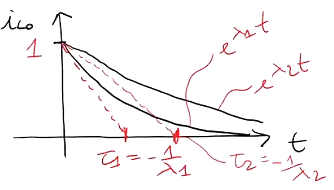
\includegraphics[width=0.4\linewidth]{evoluzione_libera_reali_distinte}
\end{figure}


\item Caso 2, radici reali e coincidenti, caso piuttosto patologico
la radice viene determinata con $-\sigma$ si avrà un modo esponenziale decrescente $e^{-\sigma t} $ con
$\tau = \frac{1}{\sigma}$ e un modo pari a  $t\cdot e^{-\sigma t}$
$$
i_{L_0} = K_1 e^{-\sigma t} + K_2 t\cdot e^{-\sigma t}
$$
\begin{figure}[H]
\centering
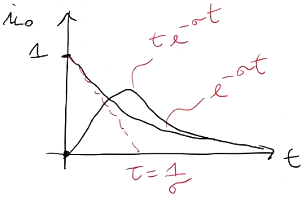
\includegraphics[width = 0.4\linewidth]{evoluzione_libera_reali_coincidenti}
\end{figure}
Vengono detti modi aperiodici smorzati con smorzamento critico.


\item Caso 3, modi periodici smorzati, soluzioni complesse coniugate
$\lambda_{1,2} = -\sigma \pm j\omega_d$, la distanza tra due picchi è pari a $\frac{2\pi}{\omega_d}$
$$i_{L_0}(t) = e^{-\sigma t} [K_1 \cos (\omega_d t) + K_2 \sin(\omega_d t)]$$
\begin{figure}[H]
\centering
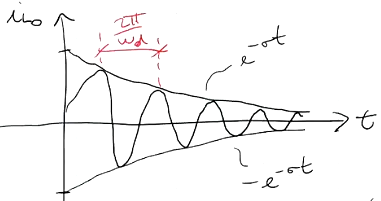
\includegraphics[width=0.4\linewidth]{evoluzione_libera_complesse_coniugate}
\end{figure}
\end{itemize}

Restano da determinare le costanti di integrazione imponendo le condizioni iniziali,
\begin{equation*}
\begin{cases}
i_L(0^+) = i_L(0^-) = \SI{0}{\ampere}\\
\frac{di_L}{dt}(0^+) = \frac{1}{L}[v_C(0^+) - R_2i_L(0^+)] = 0
\end{cases}
\end{equation*}

Supponendo dunque di avere soluzioni $\lambda_1,\ \lambda_2$ reali e distinte e ricordando di aggiungere
il termine a regime $\frac{E}{R_1 + R_2}$ nella determinazione dei coefficienti
$$
\begin{aligned}
i_L(0^+) = 0 & \Rightarrow \\
\frac{di_L}{dt}(0^+) = 0 & \Rightarrow
\end{aligned}
\begin{cases}
K_1+K_2 + \frac{E}{R_1+R_2} = 0 \\
\lambda_1K_1 + \lambda_2K_2 = 0
\end{cases}
$$
La soluzione del sistema permette di ricavare i coefficienti $K_1$ e $K_2$

%Lezione 2 i minuti si riferiranno a quelli visibili su teams e non quelli del file registrato con OBS
\section{Determinazione equazioni di stato di un circuito qualsiasi}

Si riprende la classe di circuiti lineari tempo invarianti (LTI), supponiamo di conoscere
le variabili di stato $i_L(t) $ e $v_C(t) $ assumendole note, sostituiamo ogni \textit{condensatore}
con un generatore di tensione di valore pari alla $v_C(t)$ , ripetendo il procedimento
per ciascun \textit{induttore} che viene sostituito con un generatore di corrente con corrente impressa
pari a $i_L(t)$.

In queste condizioni, la soluzione del circuito resta formalmente invariata.
Il nuovo circuito sarà di tipo adinamico, non presenterà più alcun componente dinamico, il nuovo circuito
prende il nome di \textit{circuito resistivo associato al circuito di partenza}.

Il vantaggio di questa operazione è la possibilità di ricavare $v_L$ e $i_C$ utilizzando il principio
di \textit{sovrapposizione degli effetti} (PSE).

Si ricavano le equazioni di stato per il seguente circuito:
26:07

\begin{figure}[h]

\end{figure}

Si applica il PSE, per trovare $i_C$ e $v_L$:
$$
i_C = i_c' + i_C'' + i_C '''
$$
$$
v_L = v_L' + v_L'' + v_L'''
$$

Disegna circuiti 28:48

Circuito 1)
$$
v_L' = 0;\ i_C' = \frac{E}{R_1} 
$$
Circuito 2)
$$
i_C'' = -\frac{v_C}{R_1};\ v_L'' = v_C
$$
Circuito 3)
$$
i_C''' = -i_L;\ v_L''' = -R_2\cdot i_L
$$

Sommando i tre contributi:
$$
i_C = \frac{E}{R_1} - \frac{v_C}{R_1} - i_L = C\frac{dv_C}{dt}
$$
$$
v_L = v_C - R_2\cdot i_L = L\frac{di_L}{dt}
$$
con le condizioni di continuità delle variabili di stato:
$$
i_L(0^+) = i_L(0^-)
$$
$$
v_C(0^+) = v_C(0^-)
$$

\section{Circuiti lineari con generazioni impulsivi}
Si analizza ora un circuito che presenta generatori di tipo impulsivo, ad esempio la risposta di 
una linea elettrica a seguito di una fulminazione.
Si definisce quindi l'impulso rettangolare di ammpiezza $\Delta$, la funzione viene chiamata 
$\Pi_\Delta(t)$,(funzione porta) è costante nell'intervallo $[-\frac{\Delta}{2},\frac{\Delta}{2}]$,
l'area del rettangoloide sotteso alla funzione è pari a
$$
\int_{-\Delta/2}^{\Delta/2}\Pi_\Delta(\tau)d\tau = 1\ \forall\ \Delta \in\ ]0,+\infty[
$$
Ha senso considerare la successione di funzioni ottenute per valori $\Delta$ decrescenti,
ma dimezzando la base, per mantenere l'area unitaria, va raddoppiata l'altezza.

Passando al limite per $\Delta \rightarrow 0^+$ la successione tende in maniera non ordinaria
ad un limite che non è una funzione ma può essere definita come funzione generalizzata,
ossia distribuzione, che prende il nome di \textbf{Delta di Dirac} ($\delta(t)$).

Proprietà della delta:
\begin{itemize}
\item È nulla $\forall t \neq 0$
\item Ha integrale unitario
\item Proprietà di campionamento $\int_{-\infty}^{+\infty}f(\tau)\delta(\tau-t_0)d\tau = f(t_0)$
\end{itemize}
Esempio della proprietà di campionamento: 49:03
$$
\int_{-\Delta/2}^{\Delta/2} f(\tau)\Pi_\delta(\tau-t_0)d\tau = \frac{1}{\Delta} \int_{-\Delta/2}^{\Delta/2}  f(\tau)d\tau = f(\vartheta^*)
$$


Analizziamo un'altra funzione $U_\Delta(t)$ definita come segue:
\begin{equation*}
\begin{cases}
0\ ,& t  < -\frac{\Delta}{2} \\
1\ ,& t  > \frac{\Delta}{2} \\
\frac{1}{2}+\frac{t}{\Delta}\ ,& -\frac{\Delta}{2} \leq t \leq \frac{\delta}{2}
\end{cases}
\end{equation*}
Rampa 55:03

Eseguendo la derivata temporale si otterrà la funzione $\Pi_\Delta(t)$, al limite di $\Delta \rightarrow 0$
si ottiene la funzione definita ``gradino'' o funzione di Heaviside $u(t)$.

Un ulteriore modo per definire la $\delta(t)$ è appunto quella di derivata della funzione gradino $u(t)$.
$$
\delta(t) = \frac{d}{dt}u(t) \Leftrightarrow \int_{-\infty}^t \delta(\tau)d\tau = u(t)
$$

\paragraph{Esempio con generatore impulsivo}
Si prenda un circuito RC serie 01:12:00 e una funzione $e(t)$ che vale $E_0$ per $0 < t < T$ e $0$ 
altrimenti.
Ricaviamo $v_C(t)$:

Si suppone che la condizione iniziale, ossia per $t < 0 $, la tensione sul condensatore sia nulla.

\begin{equation*}
\begin{cases}
e(t) &= RC\frac{dv_C}{dt} + v_C \\
v_C(0) &= 0
\end{cases}
\end{equation*}

$$
\begin{cases}
E_0 &= RC\frac{dv_C}{dt} + v_C \\
v_C^{(1)}(0) &= 0 \\
0 \leq t \leq T
\end{cases}
$$

$$
\begin{cases}
0 &= RC\frac{dv_C}{dt} + v_C \\
v_C^{(2)}(0) &= v_C^{(1)}(T) \\
t \geq T
\end{cases}
$$
Rivedi 1:19:00

Si ottiene una funzione esponenziale crescente fino a $T$ e poi decrescente fino a 0 all'infinito.
Diminuendo il valore di $T$ si vede che il ``picco'' della funzione sarà più basso, al limite 
di $T \rightarrow 0$ la soluzione si annulla.
Se imponiamo il prodotto $E_0\cdot T = 1$ ed eseguiamo il limite invece:
$$
\lim_{T\rightarrow0^+} v_C(t)
$$
Supponiamo di sviluppare la funzione esponenziale con la sua serie di Taylor:
$$
e^x = 1 + x + \frac{x^2}{2!} + \frac{x^3}{3!} + ... \Rightarrow 1-e^{-\frac{t}{\tau}} \simeq \frac{t}{\tau} 
$$

$$
\begin{cases}
0\ & t\leq 0 \\
\frac{1}{T}\frac{t}{\tau}\  & 0 \leq t\leq T \\
\frac{1}{T}\frac{T}{\tau} e^{-\frac{t-T}{\tau}}\ & t\geq T
\end{cases}
$$
Per $T\rightarrow 0^+$
$$
\begin{cases}
0\ & t\leq 0\\
\frac{1}{\tau}e^{\frac{-t}{\tau}}\ & t \geq 0
\end{cases}
$$

Il primo tratto dell'equazione si approssima quindi ad un tratto lineare fino a T, arrivando ad 
un'altezza di $\frac{1}{\tau}$ vedi figura 1:32:00

Se 
$$\Pi_\Delta(t) \stackrel{\Delta\rightarrow0^+}{\rightarrow} \delta(t) \Rightarrow v_C(t) \rightarrow h(t)$$
$h(t)$ è chiamata risposta all'impulso del circuito dinamico.

$$
\delta(t) = RC\frac{dv_C}{dt} + v_C \Leftarrow i_C = \frac{\delta(t)-v_C}{R}
$$
Se la tensione è impulsiva anche la corrente nel condensatore sarà di tipo impulsivo
$$
i_c = C\frac{dv_C}{dt} \Rightarrow \int_{0^-}^{0^+} i_C(\tau)d\tau = e[v_C(0^+)-v_C(0^-)]
$$
$$
v_C(0^+) - v_C(0^-) = \frac{1}{RC} \int_{0^-}^{0^+} \delta(\tau)d\tau - \frac{1}{RC} \int_{0^-}^{0^+} v_C(\tau)d\tau = \frac{1}{RC} = \frac{1}{\tau} \Rightarrow 
$$
$$
\Rightarrow v_C(0^+) = \frac{1}{RC} = \frac{1}{\tau}
$$
Rivedi discorso potenza 1:44:00

\paragraph{Risposta al gradino unitario di un circuito dinamico LTI}
Stesso circuito del precedente, ma stavolta si utilizza come forzamento il gradino unitario di
Heaviside, la soluzione è più semplice della precedente:

$$
v_C(t) = 1-e^{-\frac{t}{\tau}}u(t)
$$
la chiamiamo $g(t)$ e affermiamo che sia la risposta al gradino, richiamiamo la relazione
tra la funzione $\Pi_\Delta(t)$ e $U_\Delta(t)$ si ha che:
$$
\Pi_\Delta(t) = \frac{U_\Delta\left(t+\frac{\Delta}{2}\right)-U_\Delta\left(t-\frac{\Delta}{2}\right)}{\Delta} = e(t)
$$
per $\Delta \rightarrow 0^+$ ottengo $h(t) = v_C(t)$.

Essendo il circuito tempo invariante, si può trovare la risposta alla funzione $\Pi_\Delta(t)$
come combinazione lineare delle risposte delle due $U_\Delta$ opportunamente traslate, ossia
la risposta al gradino traslata.
$$
\text{Risp} \Pi_\Delta(t) = \frac{\text{Risp}\left\{U_\Delta\left(t+\frac{\Delta}{2}\right)\right\} - 
\text{Risp}\left\{U_\Delta\left(t-\frac{\Delta}{2}\right)\right\}}{\Delta} = 
\frac{g\left(t+\frac{\Delta}{2}\right) - g\left(t-\frac{\Delta}{2}\right)}{\Delta}
$$
Tutto si trasforma nella funzione rapporto incrementale della funzione $g(t)$ ossia
$$
\lim_{\Delta\rightarrow0^+}\text{Risp}\left\{\Pi_\Delta(t)\right\} = h(t) = \frac{dg}{dt}
$$

$$
h(t) = \frac{dg}{dt} = 0,\ t < 0;\ \frac{1}{\tau}e^{-\frac{t}{\tau}},\ t\geq0 
$$
La risposta all'impulso è quindi la derivata della risposta al gradino.

Si consideri un circuito RC serie
\begin{figure}[H]\centering
\begin{circuitikz}
\draw
(0,0) to [voltage source,invert,l=$u(t)$] (0,2)
      to [R=$R$] (2,2)
      to [C,l_=$C$,v^=$v_C$] (2,0) -- (0,0)
;
\end{circuitikz}
\end{figure}
si suppone che la tensione imposta al generatore sia un gradino unitario $u(t)$,
l'equazione di stato sarà:
$$
\begin{cases}
u(t) = RC \frac{dv_C}{dt} + v_C \\
v_C(0^+) = 0
\end{cases}
\Rightarrow v_C(t) = \left.
\begin{cases}
0 & t<0 \\
1-e^{-\frac{t}{\tau}} & t\geq 0
\end{cases}\right] = g(t)
$$

Si considera la funzione $U_\Delta$
$$U_\Delta(t) = 
\begin{cases}
0 & t< -\frac{\Delta}{2}\\
\frac{1}{2} + \frac{t}{\Delta} & -\frac{\Delta}{2} < t < \frac{\Delta}{2} \\
1 & t > \frac{\Delta}{2}
\end{cases}
$$
se si esegue la differenza di due funzioni $U_\Delta$ traslate di $\pm\frac{\Delta}{2}$ si ottiene 
una porta trapezoidale
$$
f(t) = \frac{U_\Delta\left(t+\frac{\Delta}{2}\right) - U_\Delta\left(t-\frac{\Delta}{2}\right)}{\Delta}
$$
tende ad una $\delta(t)$ delta di Dirac per $\Delta \rightarrow 0$.
Semplicemente si può invece definire la porta come differenza di due gradini traslati, in questo modo
si elimina il problema dei segmenti obliqui.

La linearità del sistema e la tempo-invarianza delle grandezze dei bipoli implica che la
risposta ad una combinazione lineare di funzioni traslate nel tempo si ottiene come combinazione lineare 
delle risposte dei singoli termini traslati.
$$
\text{Risp}\left\{\Pi_\Delta(t)\right\} = \frac{\text{Risp}\left\{u\left(t+\frac{\Delta}{2}\right) \right\} -\text{Risp}\left\{ u\left(t-\frac{\Delta}{2}\right) \right\}}{\Delta} = \frac{g\left(t+\frac{\Delta}{2}\right)-
g\left(t-\frac{\Delta}{2}\right)}{\Delta}
$$
Eseguendo il limite per $\Delta\to 0^+ $ si vede che quello appena presentato è un rapporto incrementale e
quindi
$$
\lim_{\Delta\to0^+} \Rightarrow \text{Risp} \left\{\delta(t)\right\} =h(t) = \frac{dg}{dt}
$$
Ricordando le funzioni $h(t)$ e $g(t)$ si vede la relazione
$$
h(t) = \begin{cases}
0 & t<0\\
\frac{1}{\tau}e^{-\frac{t}{\tau}} & t\geq 0
\end{cases}\qquad
g(t) = \begin{cases}
0 & t<0\\
1 - e^{-\frac{t}{\tau}} & t\geq 0
\end{cases} \Rightarrow
\frac{dg}{dt} = h(t)
$$
è possibile studiare la risposta all'impulso sfruttando quella al gradino, che è una funzione limitata e 
più semplice da analizzare.

\paragraph{Circuiti RC ed RL semplici con generatori impulsivi}
Si considerino 2 circuiti modello: il circuito RC parallelo e il circuito RL serie.

\begin{figure}[H]\centering
\begin{subfigure}{.4\textwidth}\centering
\begin{circuitikz}
\draw
(0,0) to [current source,l=$j(t)$] (0,2)
      to (1,2) to [R=$R$,i>^=$i_R$] (1,0) to (0,0);
\draw
(1,2) to (2.5,2)  to [C,l_=$C$,v^=$v_C(t)$,i>_=$i_C$] (2.5,0) -- (1,0)
;
\end{circuitikz}
\subcaption{RC parallelo}
\end{subfigure}
\begin{subfigure}{.4\textwidth}\centering
\begin{circuitikz}
\draw
(0,0) to [voltage source,invert,l=$e(t)$] (0,2)
      to [R,l_=$R$] (2.5,2) to [L,l_=$L$,i_>=$i_L(t)$,v^=$v_L$] (2.5,0) -- (0,0)
;
\end{circuitikz}
\subcaption{RL serie}
\end{subfigure}
\end{figure}

Siano i generatori impulsivi: $j(t) = Q\delta(t)$ ed $e(t) = \Phi\delta(t)$.
$$
j(t) = \frac{v_C}{R} + i_C = Q\delta(t) = \frac{v_C}{R} + C\frac{dv_C}{dt}
$$
Si integra la funzione nell'istante in cui è centrata la $\delta(t)$ ossia:
$$
\int_{0^-}^{0^+} Q\delta(\tau)d\tau  = \cancel{\int_{0^-}^{0^+}\frac{v_C}{R}d\tau} + C[v_C(0^+)-\cancel{v_C(0^-)}]
\Leftrightarrow Q = Cv_C(0^+) \ \ [Q] = \si{\coulomb} \text{ (Coulomb)}
$$
$$
\left[\int_{0^-}^{0^+} Q\delta(\tau)d\tau\right] = \text{ Coulomb}
$$
Tirando la costante $C$ fuori dall'integrale, che ha la dimensione di Coulomb, l'integrale rimanente
deve essere adimensionale.
Ciò significa che la $\delta(t)$ ha la dimensione di \si{\per\second} per essere coerente con l'integrale
e restituire una quantità finita.

\subparagraph{Caso duale con circuito RL:}

$$
e(t) = R\cdot i_L + v_L
$$
$$
\Phi\delta(t) = R\cdot i_L + L\frac{di_L}{dt}
$$
$$
\Phi\int_{0^-}^{0^+} \delta(\tau)d\tau = L i_L(0^+)\ , \ i_L(0^-) = 0
$$

Anche in questo caso per avere la dimensione del flusso in \si{\weber} per $\Phi$ allora la $\delta(t)$ 
avrà le dimensioni di \si{\per\second}.
\newpage
\subsection{Procedura generale per la risoluzione di circuiti con generatori impulsivi}
Si ha un circuito dinamico semplice al quale è collegato un generatore impulsivo,
si determina il circuito resistivo associato, ossia vengono sostituiti i condensatori con 
generatori di tensione e gli induttori con generatori di corrente.

Si ottiene un circuito parziale in cui si spengono i generatori interni (anche quelli equivalenti ai bipoli dinamici) e si lascia agire solo il generatore impulsivo.

Un ulteriore circuito è ottenuto facendo l'esatto contrario e spegnendo quindi il generatore impulsivo.

\begin{figure}[H]\centering
\begin{subfigure}{0.45\linewidth}\centering
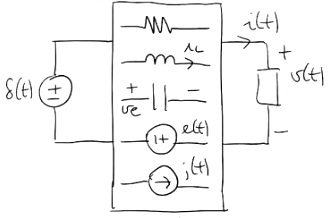
\includegraphics[width=\linewidth]{lezione_03_circuito_A}
\subcaption{Circuito iniziale}
\end{subfigure}
\begin{subfigure}{0.45\linewidth}\centering
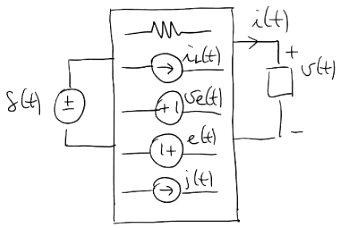
\includegraphics[width=\linewidth]{lezione_03_circuito_B}
\subcaption{Circuito resistivo associato}
\end{subfigure}
\begin{subfigure}{0.45\linewidth}\centering
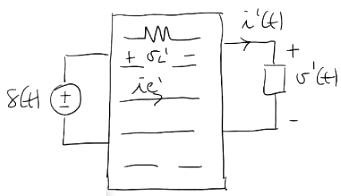
\includegraphics[width=\linewidth]{lezione_03_circuito_C-}
\subcaption{Circuito C'}
\end{subfigure}
\begin{subfigure}{0.4\linewidth}\centering
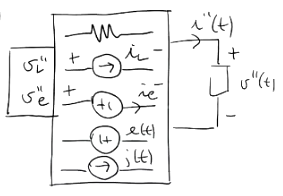
\includegraphics[width=\linewidth]{lezione_03_circuito_C--}
\subcaption{Circuito C"}
\end{subfigure}
\end{figure}
37:19
Si applica il PSE (Principio di Sovrapposizione degli effetti)
$$
\begin{cases}
v_L = v_L' + v_L''\\
i_C = i_C' + i_C''
\end{cases}
$$

Dal circuito C' si ricavano $v_L'$ e $i_C'$ causate dai generatori impulsivi 41:41

Viceversa dal circuito C'' si valutano le variabili di stato utilizzando come condizioni iniziali
le variabili ottenute in C'.

$$
v_C(0^+) = \frac{1}{C} \int_{0^-}^{0^+} i_C'(\tau)d\tau \ , \ v_C(0^-) = 0
$$
$$
i_L(0^+) = \frac{1}{L} \int_{0^-}^{0^+} i_L'(\tau)d\tau \ , \ i_L(0^-) = 0
$$
L'integrale delle variabili di stato del circuito C'' è pari a 0 dato che la funzione integranda è limitata
e l'intervallo è infinitesimo.

Infine si risolve il circuito C'' usando le variabili di stato appena calcolate in C'.

Esercizio 

Conclusione dell'esercizio: le variabili di stato possono essere discontinue ma limitate, le altre
variabili possono invece essere anche impulsive.

\paragraph{Risposta forzata di un circuito LTI}
Si suppone di avere un solo generatore esterno, se ne vogliono determinare le variabili ai capi
di un solo bipolo, si parla di filtro o sistema SISO \textit{(Single Input Single Output)},
sia $x(t)$ l'ingresso e $y(t)$ l'uscita, si deve supporre che il circuito sia a stato 0, ossia
le sue variabili di stato sono tutte nulle (circuito precedentemente spento).

Si parla di approssimazione \textit{PieceWise-Constant} ossia costante a tratti dell'ingresso
$x(t)$.
Si partiziona l'asse dei tempi in tanti intervalli di ampiezza $\Delta t$ centrati negli istanti
di tempo $t_k = k\Delta t\ ,\ k\ \in\ Z$.

Costruiamo un'approssimazione $x_\Delta(t)$ costante di valore $x(t_k)$ in $\left[t_k-\frac{\Delta t}{2}\ ,\ 
t_k+\frac{\Delta t}{2}\right]$.
La funzione $x(t)$ può quindi essere rappresentata come somma di impulsi rettangolari successivi,
sfruttando la funzione $\Pi_{\Delta}(t)$, sarà quindi:
$$
x_{\Delta}(t) = \sum_{k = -\infty}^{+\infty} x(t_k) \Pi_\Delta(t-t_k)\Delta t
$$
Eseguendo il limite per $\Delta t \rightarrow 0^+$ in ipotesi di sufficiente regolarità:
$$
\lim_{\Delta t \to 0^+} x_\Delta(t) = x(t) = \int_{-\infty}^{+\infty} x(\tau) \delta (t-\tau)
d\tau
$$
Questa conclusione richiama la proprietà di campionamento della $\delta(t)$.

Se vogliamo calcolare la risposta di $x(t)$ allora:
$$
\text{Risp}\left\{x(t)\right\} = y(t) = \text{Risp} \left\{\int_{-\infty}^{+\infty} x(\tau)\delta(t-\tau)
d\tau\right\}
$$
per linearità e tempo-invarianza si ottiene
$$
y(t) = \int_{-\infty}^{+\infty} x(\tau)h(t-\tau) d\tau
$$
chiamato integrale di convoluzione, $h(t)$ è la risposta impulsiva per la variabile di uscita.

Si parla di prodotto di convoluzione tra due funzioni $f,g \ \in\ R$
$$
f * g(t) = \int_{-\infty}^{+\infty} f(\tau)g(t-\tau)d\tau
$$
Si può calcolare la risposta impulsiva... rivedi 1:57:00


Data la risposta all'ingresso impulsivo, si può calcolare la risposta a qualsiasi ingresso, mediante
l'uso dell'integrale di convoluzione.
Osservando attentamente l'integrale si vede che la risposta impulsiva gode della proprietà per la quale
$$
h(t) = 0 \ t<0,\ h(t) \neq 0 \forall t\ \geq 0 \Rightarrow t - \tau \geq 0 \Rightarrow \tau \leq t
$$

Se l'ingresso $x(t) = 0,\ t< t_0$ allora possiamo affermare che la $y(t)$ avrà come estremi di integrazione
$t_0^-$ e $t$, con il - si sottintende la possibilità che siano presenti $\delta(t_0)$ in quell'istante 
di tempo.

\paragraph{Esempi dell'utilizzo dell'integrale di convoluzione}
Circuito RC parallelo con forzamento esponenziale, forzato da un generatore di corrente.
$$
j(t) = I e ^{\frac{t}{\tau}} u(t)
$$
Per studiare la risposta del circuito bisogna per prima cosa determinare la $V_{cf}(t)$, mediante
lo studio della risposta impulsiva.
Per determinare la risposta impulsiva si forza il circuito con una $\delta(t)$, utilizzando i metodi 
precedenti.

$i_c = \delta(t)$
$$
v_c(0^+) = \frac{1}{C}\int_{0^-}^{0^+} i_c(\tau)d\tau + V_c(0^-) = \frac{1}{C}
$$
Per determinare la risposta impulsiva si determina l'evoluzione libera spegnendo il generatore,
ci sarà un parallelo RC con la seguente equazione di stato:
$$
\begin{cases}
RC\frac{dV_c}{dt} + v_C = 0 \\
V_c(0^+) = \frac{1}{C}
\end{cases}
$$
Quindi 
$$
V_{c_{lib}} = h(t) = \frac{1}{C} e^{-\frac{t}{RC}},\ t\geq 0
$$
$$
h(t) = \frac{1}{C}e^{-\frac{t}{RC}}\cdot u(t) \forall t
$$

Utilizzando l'integrale di convoluzione per calcolare la risposta forzata:

$$
V_{cf}(t) = \int_{0^-}^{t}Ie^{\frac{\tau}{T}} \cdot \frac{1}{C} e^{-\frac{t-\tau}{RC}} d\tau = 
\frac{I}{C} \int_{0^-}^{t} e^{\frac{\tau}{t}}\cdot e^{-\frac{t}{RC}}\cdot e^{\frac{\tau}{RC}} d\tau
$$

$$
= \frac{I}{C} e^{-\frac{t}{RC}}\cdot \frac{e^{t\left(\frac{1}{T}+\frac{1}{RC}\right)}-1}{\frac{1}{RC}+\frac{1}{T}}
$$

Circuito RC serie con forzamento in tensione a rampa lineare $e(t)$
$$
e(t) = \begin{cases}
0\ t<0 \\
\frac{t}{T},\ 0\leq t\leq T\\
0\ t>0
\end{cases}
$$
Possiamo rappresentare questa funzione mediante l'uso di due funzioni $u(t)$

$$
e(t) = \frac{t}{T}\left[u(t) - u(t-T)\right]
$$
Determiniamo quindi la risposta $h(t)$ mediante la risposta al gradino $g(t)$
Le equazione di stato è:
$$
\begin{cases}
1 = RC\frac{dV_c}{dt} + V_c \\
V_c(0) = 0 
\end{cases}
\Rightarrow V_c(t) = 1 - e^{-\frac{t}{RC}},\ t\geq 0$$
Quindi 
$$
g(t) = (1 - e^{-\frac{t}{RC}})u(t) \forall t
$$
ma
$$
h(t) = \frac{dg}{dt} = \frac{1}{RC}e^{-\frac{t}{RC}},\ t\geq 0
$$
Determiniamo ora la risposta forzata $v_{cf}(t)$:
$$
V_{cf}(t) = \int_{0^-}^{t} e(\tau) h(t-\tau)d\tau = \int_{0^-}^{t}\frac{\tau}{T}\left[u(\tau) - u(t-\tau)\right]
\cdot \frac{1}{RC} e ^{-\frac{t-\tau}{RC}}\cdot u(t-\tau)d\tau
$$
Svolgiamo ora l'integrale osservando che $e(\tau) \neq 0 $ solo se $t \in [0,T]$, separiamo quindi
il calcolo dell'integrale in due eventualità:
$$
t\leq T:\ \int_{0^-}^{t}\frac{\tau}{T}\frac{1}{RC}e^{-\frac{t-\tau}{RC}}d\tau = \frac{1}{TRC}e^{-\frac{t}{RC}}\int_{0^-}^{t}\tau e^{\frac{\tau}{RC}}d\tau 
$$
utilizzando l'integrazione per parti:
$$
\left(f\cdot g\right)' = f'g + g'f
$$
$$
f = \tau\ g' = e^{\frac{\tau}{RC}}
$$
$$
\frac{1}{TRC}e^{-\frac{t}{}RC}\int_{0^-}^{t}\frac{d}{dt}\left[\tau e^{\frac{\tau}{RC}}\cdot RC \right] -
RC e^{\frac{\tau}{RC}} d\tau =
$$
$$
\frac{1}{TRC} e^{-\frac{t}{RC}} \left\{ \left[t e^{\frac{t}{RC}}\cdot RC \right] - \left[(RC)^2 e^{\frac{\tau}{RC}} \right]_{0^-}^{t}  \right\} =
$$
$$
\frac{t}{T} - \frac{RC}{T}\left(1-e^{-\frac{t}{RC}}\right)
$$

Secondo caso:
$$
t > T:\ \int_{0^-}^{T} \frac{\tau}{T}\frac{1}{RC} e^{-\frac{t-\tau}{RC}}d\tau =  e^{-\frac{t-T}{RC}}-\frac{RC}{T}\left(e^{-\frac{t-T}{RC}} -e^{-\frac{t}{RC}} \right)
$$

\section{La trasformata di Laplace}
Il metodo dei fasori si basa sul concetto che conoscendo l'andamento di regime con grandezze isofrequenziali, si può risolvere il sistema traspotando le grandezze sinusoidali nel dominio simbolico
dei fasori, si rapprentano cioè le grandezze descrittive dei bipoli medianti numeri complessi.

Mediante la L-Trasformata si possono usare ancora una volta equazioni nel dominio complesso ma per 
studiare reti nel regime transitorio.

\paragraph{Analisi delle reti dinamiche LTI con Laplace}
Consideriamo un blocco contenenti tutte le equazioni circuitali nel dominio del tempo,
otteniamo tutte le equazioni di stato di induttori e condensatori.
Questo risultato si ottiene mediante i metodi di risoluzione delle ODE, per arrivare alla conoscenza
della dinamica delle \textit{variabili di stato}, se sono poi interessato ad altre variabili, attravarso
operazioni \textit{algebriche lineari} si conosce la dinamica di utte le variabili del circuito.

In alternativa, sfruttando la trasformata di Laplace, le equazioni ODE vengono trasformate nel dominio
di Laplace, saranno equazioni algebriche lineari anzichè differenziali, risolvendo quindi solo un sistema
di equazioni lineari si conosce direttamente la trasformata delle variabili di stato, effettuando quindi
il procedimento inverso di antitrasformazione si ricavano le variabili di stato nel dominio del tempo,
l'antitrasformazione può essere invece posticipata ed eseguita dopo aver ricavato le generiche variabili
del circuito, ancora una volta con operazioni algebriche.

La soluzione di un sistema di equazioni differenziali è notevolmente più complesso che risolvere un 
sistema lineare, ecco il vantaggio dell'utilizzo della trasformata di Laplace.

Definizione della trasformata di Laplace di una funzione $f(t)\ \in\ [0,+\infty[\to R$:
$$
L[f(t)] = F(s) = \int_{0^-}^{+\infty} f(t) e^{-st}dt \ F:s \in\ C \to C
$$
ammesso che l'integrale improprio converga, per assicurarci che ciò accade si pone la condizione sufficiente, verificata nella stragrande delle situazioni:
$$
\text{Se} \left|f(t) \right| \leq Me^{\alpha t} ,\ M,\alpha \in R \text{ costanti}
$$
allora l'integrale converge, dim.:
$$
\int_{0^-}^{+\infty} f(t) e^{-st}dt \leq \int_{0^-}^{+\infty} \left|f(t)\right| e^{-st}dt \leq
\int_{0^-}^{+\infty} Me^{\alpha t} e^{-st}dt = M\int_{0^-}^{+\infty} e^{(\alpha-s)t}dt
$$
condizione verificata per ogni $\Re \left\{ s\right\} > \alpha$.

Definizione dell'antitrasformata:
$$
L^{-1}\left[F(S) \right] = f(t) = \frac{1}{2\pi i} \lim_{T\to+\infty} \int_{\gamma-iT}^{\gamma+iT}
e^{st}F(s)ds
$$
con $\Re\left\{s\right\} = \gamma$ tale che tutte le singolarità di $F(s)$ si trovino a sinistra di $\gamma$.

\subsection{Proprietà della L-trasformata} Ricordando quelle utilizzate nel metodo dei fasori:
\begin{itemize}
\item Unicità: $\forall f(t) \in [0,+\infty[\ \exists!\ F(s) = L[F(s)]$

considerate $F(s)$ e $G(s)$, se $F(s) = G(s) \Rightarrow f(t) = g(t)$ quasi ovunque, ossia:
$$\int_{0^-}^{+\infty}|f(t) - g(t)|dt = 0$$

\item Linearità: date $f_1(t)$ ed $f_2(t) :\ [0,+\infty[ \rightarrow R,\ k_1,k_2 \in R$ allora
$$L[k_1f_1(t) + k_2f_2(t)] = k_1F_1(s) + k_2F_2(s) $$
si dimostra con la proprietà di linearità dell'integrale

\item Traslazione nel dominio di Laplace: sia data $f(t) \in [0^-,+\infty[,\ L[f(t)] = F(s)$ e
consideriamo $F(s-\lambda),\ \lambda\ \in\ C$ 
$$F(s-\lambda) = \int_{0^-}^{+\infty}f(t) e^{-(s-\lambda)t}dt = \int_{0^-}^{+\infty} (f(t)e^{\lambda t})e^{-st} dt \Rightarrow F(s-\lambda) = L[f(t) e^{\lambda t}]$$ con $\Re\{s\} > \lambda$ 

\item Derivazione: $f'(t)  = \frac{d}{dt}f(t),\ L[f(t)] = F(s)$ allora 
$$L\left[\frac{d}{dt}f(t)\right] = \int_{0^-}^{+\infty}f'e^{-st}dt \stackrel{\text{x parti}}{=} 
\left[fe^{-st}\right]_0^{+\infty} - \int_{0^-}^{+\infty}(-s)e^{-st}\cdot f dt =$$
$$= \left(\lim_{t\to\infty}\left[fe^{-st}\right]-f(0^-)\right) + sF(s) = sF(s) - f(0^-)$$
$$
L\left[\frac{d}{dt}f(t)\right] = sF(s) - f(0^-)
$$
\item Prodotto di convoluzione nel dominio di Laplace, facendo leva sul teorema di Borel:
$$
L\left[f*g(t)\right] =\int_{0^-}^{+\infty}\left(\int_{0^-}^{t}f(\tau)g(t-\tau)d\tau\right) e^{-st}dt = F(s)\cdot G(s)
$$
per dimostrare questo teorema si scambiano le variabili di integrazione $t$ e $\tau$ sfruttando i teoremi
di \href{https://it.wikipedia.org/wiki/Teorema_di_Fubini}{Fubini} e Tonelli
\end{itemize}
\newpage
Trasformate notevoli di frequente utilizzo nei circuiti:
\begin{itemize}
\item Esponenziale: $f(t) = e^{\lambda t},\ \lambda\ \in R $ 
$$
L\left[e^{\lambda t}\right] = \int_{0^-}^{+\infty} e^{-(s-\lambda) t} dt = \left[\frac{1}{\lambda -s}e^{(\lambda -s)t}\right]_{0^-}^{+\infty} = \frac{1}{\lambda -s} \left[\lim_{t\to\infty}e^{(\lambda-s)t}-1\right] =
\frac{1}{s-\lambda}
$$
\item Funzione gradino $u(t)$:
$$
L[u(t)] = \int_{0^-}^{+\infty}e^{0t}e^{-st}dt = \frac{1}{s}
$$
\item Delta di Dirac $\delta(t)$:
$$
L[\delta(t)] = \int_{0^-}^{+\infty}\delta(t) e^{-st}dt = e^{-s\cdot 0} = 1
$$
\item Funzioni sinusoidali, $\cos(\omega t)=\frac{e^{j\omega t}+e^{-j\omega t}}{2},\ \sin(\omega t) = \frac{e^{j\omega t}-e^{-j\omega t}}{2j}$
$$
L[\cos(\omega t)] = \frac{1}{2} L[e^{j\omega t}] + \frac{1}{2} L[e^{-j\omega t}] = \frac{s}{s^2+\omega^2},\ \Re\{s\} > 0
$$
$$
L[\sin(\omega t)] = \frac{1}{2j}\left(\frac{1}{s-j\omega}-\frac{1}{s+j\omega}\right) = \frac{\omega}{s^2+\omega^2},\ \Re\{ s\} > 0
$$
\end{itemize}


Funzioni generiche: $t\cdot f(t)$ con $f(t)$ le funzioni precedentemente analizzate.
\begin{itemize}
\item Esponenziale:
$$
L[te^{\lambda t}] = \int_{0^-}^{+\infty} t e^{\lambda t}e^{-s t} dt = \int_{0^-}^{+\infty}t e^{(\lambda -s)t}
dt = 
$$
$$
= \left[\frac{e^{(\lambda -s )t }}{\lambda-s}\cdot t\right]_{0^-}^{+\infty} - \int_{0^-}^{+\infty}1\cdot\frac{1}{\lambda -s}e^{(\lambda-s)t}dt = 
$$
$$
= 0 + \frac{1}{s-\lambda}\cdot\frac{1}{s-\lambda} = \frac{1}{s-\lambda} ,\ \Re\{s\} > \lambda
$$

\item Coseno:
$$
L[t\cos(\omega t)] = L\left[t \frac{e^{j\omega t}+e^{-j\omega t}}{2}\right] = \frac{1}{2}\frac{1}{(s-j\omega)^2} + \frac{1}{2}\frac{1}{(s+j\omega)^2} = 
$$
$$
= \frac{1}{2}\frac{1}{s^2-\omega^2-2j\omega s} + \frac{1}{2}\frac{1}{s^2-\omega^2+2j\omega s} =
\frac{1}{2}\frac{s^2-\omega^2+2j\omega s +s^2 -\omega^2 -2j\omega s}{(s^2-\omega^2)^2+4\omega^4s^2} =
$$
$$
= \frac{s^2-\omega^2}{(s^2+\omega^2)^2}
$$

\item Seno:
$$%%Rivedi il rigo qui sotto
L[t\sin(\omega t)] = \frac{1}{2j} \left[\frac{1}{(s-j\omega)^2}-\frac{1}{(s+j\omega)^2}\right] =
\frac{1}{2j}\left[\frac{s^2-\omega^2+2j\omega s-s^2+\omega^2+2j\omega s}{(s^2-\omega^2)^2+4\omega^2s^2}\right] = 
$$
$$
= \frac{2\omega s}{(s^2+\omega^2)^2}
$$
\item Funzioni che descrivono moti periodici smorzati, sfruttando la proprietà di traslazione
$f(t) = e^{-\sigma t}\cos(\omega t),\  e^{-\sigma t}\sin(\omega t)$:
$$
L[e^{-\sigma t}\cos(\omega t)] = L[\cos(\omega t)](s+\sigma) = \frac{s+\sigma}{(s+\sigma)^2+\omega^2}\ \Re\{s\} > -\sigma
$$
$$
L[e^{-\sigma t}\sin(\omega t)] = L[\sin(\omega t)](s+\sigma) = \frac{\omega}{(s+\sigma)^2+\omega^2}\ \Re\{s\} > -\sigma
$$
\end{itemize}
\newpage
\paragraph{Circuito RL serie con L-trasformata}
Sia dato il circuito RL serie, se ne voglia determinare la risposta impulsiva $h(t) = i_L(t)$ dato l'ingresso
$e(t) = \delta(t)$

\begin{figure}[H]
\centering
\begin{circuitikz}
\draw (0,0) to [voltage source,invert,l=$e(t)$] (0,2)  
            to  [R,l=$R$] (2,2) to [L,i>_=$i_L$,l_=$L$,v^=$v_L$] (2,0) to (0,0);
\end{circuitikz}
\end{figure}

$$
\begin{cases}
\delta(t) = R\cdot i_L + L\frac{di_L}{dt} \\
i_L(0^-) = 0
\end{cases}
$$
Si applica la trasformata di Laplace ad entrambi i membri della prima equazione, sfruttando anche
la proprietà di derivazione:
$$
1 = RI_L(s) + L(sI_L(s) - i_L(0^-))
$$
$$
L[i_L(t)] = I_L(s) = \frac{1}{R+sL} = \frac{1}{L}\frac{1}{\frac{R}{L}+s}
$$
L'antitrasformata sarà invece pari a:
$$
L^{-1}[I_L(s)] = \frac{1}{L} L^{-1}\left[\frac{1}{S+\frac{R}{L}}\right] = \frac{1}{L}e^{-\frac{t}{\tau}},\ 
\tau = \frac{L}{R}
$$

Si vede ora la risposta al gradino, $e(t) = u(t)$:
$$
u(t) = R\cdot i_L+ L\frac{di_L}{dt} \rightarrow \frac{1}{s} = RI_L + sLI_L 
$$
$$
I_L = \frac{1}{s(R+sL)} = \frac{A}{s} + \frac{B}{R+sL} = \frac{AR+sLA+sB}{s(R+sL)}
$$
Si ricavano i valori di $A$ e $B$ sfruttando il principio di identità dei polinomi:
$$\begin{cases}
LA+B = 0\\
AR = 1
\end{cases}$$

$$
A = \frac{1}{R},\ B = -\frac{L}{R}
$$
In conclusione:
$$
I_L(s) = \frac{1}{R}\left[\frac{1}{s}-\frac{L}{R+SL}\right] = \frac{1}{R}\left[\frac{1}{s}-
\frac{L}{L\left(\frac{R}{L}+s\right)}\right]
$$
Antitrasformando si ottiene:
$$
i_L(t) = \frac{u(t)}{R} - \frac{1}{R}e^{-\frac{R}{L}t}u(t) = \frac{u(t)}{R}\left(1-e^{-\frac{R}{L}}t\right)
$$

\subsection{Equazioni circuitali nel dominio della L-trasformata}
Si considera ancora la classe dei circuiti dinamici lineari tempo-invarianti (LTI),
nel dominio del tempo sono necessarie le LKT e le LKC, le caratteristiche dei bipoli e dei generatori.
Questo sistema è un DAE (Differential Algebric Equation), va trasformato in un ODE nelle variabili di stato per poter essere risolto.

Se si trasformano tutte le equazioni che provengono dalle leggi di Kirchhoff si ottengono ancora le stesse equazioni
ma nel dominio di Laplace:
$$
\sum_{k} (\pm)I_k(s) = 0
$$
$$
\sum_k (\pm)V_k(s) = 0
$$
Ancora le equazioni dei bipoli:
$$\begin{aligned}
V_R(s) &= RI_R(s)\\
V_L(s) &= sLI_L(s) - Li_L(0^-)\\
I_C(s) &= sCV_C(s) - Cv_C(0^-)\\
V_E(s) &= E(s)\\
I_J(s)&= J(s)
\end{aligned}$$

Per trattare i circuiti in evoluzione forzata ($i_L(0^-)=0,\ v_C(0^-)=0$) si può associare un'impedenza equivalente
ai bipoli, ad esempio l'impedenza operatoriale dell'induttore diventa
$$\begin{aligned}
Z_L(s) = sL,&\ V_L(s) = Z_LI_L(s)\\
Y_C(s) = sC,&\ I_C= Y_C V_C 
\end{aligned}$$
Questo risultato permette di utilizzare tutti i metodi precedentemente visti per la risoluzione
di un circuito, si esegue un'antitrasformazione alla fine per ritornare nel dominio del tempo.
Si è però posta l'ipotesi di trovarsi in evoluzione forzata, ossia supponendo uno stato iniziale 
nullo, cosa accade se ciò non è vero?

Stato non zero iniziale:
$$\begin{aligned}
V_L(s) &= sLI_L - L i_L(0^-)\\
V_L(s) &= Z_LI_L+E_0
\end{aligned}$$
Si modella il bipolo dinamico con un generatore di tensione in serie, impulsivo.
Si può fare un ragionamento simile con il condensatore al quale si affianca un generatore di corrente
in parallelo $J_{cc}$
$$\begin{aligned}
I_C(s) &= sCV_C(s) - Cv_C(0^-)\\
J_{cc} &= Cv_C(0^-)
\end{aligned}$$

\subsection{Funzione di trasferimento e legame con la risposta impulsiva}
Sia preso un generico circuito LTI, viene forzato con un generatore di tensione, se ne analizzano
le grandezze su un singolo bipolo interno al circuito, considerato quindi come un SISO $h(t)$,
l'uscita del sistema può essere calcolata mediante l'integrale di convoluzione della risposta impulsiva.
$$
y(t) = \int_{0^-}^{t} x(\tau)h(t-\tau)d\tau
$$
Si trasporta il fenomeno nel dominio di Laplace e si considera lo stesso circuito sostituito dai bipoli
operatoriali, si può ancora considerare il sistema come un SISO con ingresso pari a $X(s)$ e uscita
pari a $Y(s)$.
Questo circuito è a-dinamico lineare con un solo generatore, quindi tutte le grandezze sono proporzionali
al singolo forzamento, si può quindi affermare che $Y(s) = H(s)X(s)$ con $H(s)$ un coefficiente di 
proporzionalità.

$H(s)$ viene ricavato, mediante il teorema di Borel:
$$
L[f*g(t)] = F(s)\cdot G(s)
$$
$$
y(t) = \int_{0^-}^{t} x(\tau)h(t-\tau) d\tau \Rightarrow H(s) = L[h(t)]
$$
$H(s)$ si chiama quindi \textit{funzione di trasferimento} del circuito ed è definita come il rapporto
tra la trasformata dell'uscita e quella dell'ingresso e coincide con la trasformata della risposta
impulsiva del circuito:
$$
H(s) \stackrel{\text{def}}{=} \frac{Y(s)}{X(s)} = L[h(t)]
$$

\paragraph{Esempio} Circuito LC forzato in risonanza:

Si ha un generatore ideale di tensione, un induttore ideale e un condensatore ideale senza perdite,
questo circuito rappresenta il limite ideale 
La risonanza è associata ad una specifica pulsazione pari a:
$$
\omega_r = \frac{1}{\sqrt{LC}}
$$
e il forzamento è pari ad un segnale con pulsazione pari alla pulsazione di risonanza
$$
e(t) = E_m \sin(\omega_r t)
$$
Il circuito non può essere analizzato con il metodo dei fasori dato che non è dissipativo e l'energia 
immagazzinata nei bipoli dinamici non tende a 0 in evoluzione libera per $t\to \infty$.

Si utilizza quindi l'analisi nel dominio di Laplace:
$$
I(s) = \frac{E(s)}{sL+ \frac{1}{SC}}
$$
ma
$$
E(s) = \frac{\omega_r}{s^2+\omega_r^2} = \frac{\omega_r}{s^2+\frac{1}{LC}} = L[e(t)]
$$
$$
I(s) = \frac{E_m\omega_r s C}{(s^2+\frac{1}{LC})(s^2+\frac{1}{LC})} = \frac{E_m\omega_r\frac{sC}{LC}}{(s^2+\frac{1}{LC})^2} = \frac{E_m\omega_r}{L} \frac{s}{(s^2+\frac{1}{LC})^2}
$$
Riprendendo la trasformata del seno:
$$
L[t\sin(\omega_r t)] = \frac{2\omega s}{(s^2+\omega^2)^2}
$$
riprendendo il calcolo di $I(s)$:
$$
= \frac{E_m\omega_r}{2L\omega_r}\cdot \frac{2\omega_r s}{(s^2+\omega_r^2)^2} = \frac{E_m}{2L}\frac{2\omega_r s}{(s^2+\frac{1}{LC})^2}
$$
Antitrasformando:
$$
i(t) = L^{-1}[I(s)] = \frac{E_m}{2L} t \sin(\omega_r t)
$$

\newpage
\paragraph{Calcolo della funzione di trasferimento per un circuito del secondo ordine}

$$R_1 = \SI{5}{\ohm}\ R_2=R_3 = \SI{10} {\ohm}\ C=\SI{0.5}{\farad}\ L=\SI{1}{\henry}$$
\begin{figure}[H]\centering
\begin{circuitikz}
\draw (0,2) to [open,v=$e(t)$] (0,0); 
\draw (0,2) to [R,l_=$R_1$] (2,2)
            to [L,l_=$L$] (4,2)
            to [R,l_=$R_2$] (4,0) to (0,0);
\draw (4,2) to (7,2)
            to [R,l_=$R_3$,v^=$v(t)$] (7,0) to (4,0);
\draw (5.5,2) to [C,l_=$C$] (5.5,0);
\end{circuitikz}
\end{figure}
Si è interessati all'uscita $v(t)$ dato l'ingresso $e(t)$, ci si trasferisce ancora una volta dal 
dominio del tempo a quello di Laplace.
Si assegnano i parametri del circuito:
$R_1 = \SI{5}{\ohm}\ R_2=R_3=\SI{10}{\ohm}\ C =\SI{0.5}{\farad}\ L=\SI{1}{\henry} $
Sostituiti i bipoli con impedenze, si trovano la $Z_{eq}$ pari a $5 + s$ in serie con $\frac{1}{0.2+0.5s}$
La tensione in uscita sarà la partizione della tensione in ingresso tra queste due impedenze:
$$
V(s) = E(s)\frac{Z_{eq}^{(2)}}{Z_{eq}^{(2)}+Z_{eq}^{(1)}} = \frac{1}{(0.2+0.5 s)(\frac{1}{0.2+0.5 s}+5+s)} = \frac{1}{2+2.75+0.5s^2}
$$
Si trovano gli zeri del polinomio, saranno due radici reali e distinte,
la $H(s)$ sarà quindi:
$$
H(s) = \frac{k_1}{s+0.886} + \frac{k_2}{s+4.514} = \frac{k_1 5 +4.514 k_1 + k_2 s + 0.886 k_2 }{s^2+5.45+4} =
$$
$$
= \frac{2}{(s^2+5s+4)},\ 
\begin{cases}k_1+k_2 = 0\\
4.514k_1 + 0.886k_2 = 2
\end{cases}
$$
$$
k_1 = \frac{2}{4.514-0.886} = 0.551 = -k_2
$$
In conclusione 
$$
H(s) = \frac{0.551}{s+0.886} - \frac{0.551}{s+4.514}
$$
antitrasformando:
$$
L^{-1}[H(s)] = 0.551\left(e^{-0.886 t}-e^{-4.514 t}\right) = h(t)
$$


\subsection{Calcolo di antitrasformate di funzioni razionali}
Si supponga che nei circuiti siano presenti soltanto alcune tipologie di generatori, come ad esempio
generatori stazionari, sinusoidali... In queste ipotesi le trasformate di Laplace sono funzioni 
razionali, del tipo:
$$
F(s) = \frac{N(s)}{D(s)}\ N(s),D(s) \text{ polinomi con grado } n\leq d
$$

In generale la $F(s)$ è esprimibile come:
$$
F(s) = K + \frac{N^*(s)}{D(s)}\ K \text{ costante, } n^* < d
$$
la sua antitrasformata sarà:
$$
L^{-1}[F(s)] = k\delta(t) + L^{-1}\left[\frac{N^*(s)}{D(s)}\right] 
$$
per determinare la soluzione vanno ricercate le radici del denominatore, chiamate \textit{poli}
della funzione, mentre le radici del numeratore vengono chiamati \textit{zeri}.

La funzione può avere \textbf{poli semplici} di molteplicità 1:
$$
F^*(s) = \frac{k_1}{s-p_1} + \frac{k_2}{s-p_2} + ... + \frac{k_n}{s-p_n} = \sum_{i=1}^{N}\frac{k_i}{s-p_i}
$$
$k_i$ viene chiamato residuo i-esimo della $F^*(s)$ e si calcola con:
\begin{equation}
\lim_{s\to p_i} \left[(s-p_1)F^*(s)\right]
\label{eq:formula_poli_semplici}
\end{equation}

Esempio:
$$
F^*(s) = \frac{1}{0.5s^2+2.7s+2} = \frac{2}{s^2+5.4s+4} = \frac{k_1}{s+0.886} + \frac{k_2}{s+4.514}
$$
Applicando la \ref{eq:formula_poli_semplici}:
$$
k_1 = \frac{2}{-0.886+4.514} = 0.551
$$
Una volta trovati tutti i poli semplici, l'antitrasformata della funzione, diviene una somma di
antitrasformate dei singoli rapporti:
$$
L^{-1}[F^*(s)] = L^{-1}\left[\sum_{i=1}^{N}\frac{k_i}{s-p_i}\right] = \sum_{i=1}^{N} k_ie^{p_i t}
$$
\textbf{Poli multipli}, ossia con molteplicità maggiore di 1, si supponga ad esempio che $p_1$ sia un polo multiplo:
$$
F^*(s) = \frac{k_{11}}{(s-p_1)^2} + \frac{k_{12}}{s-p_1} + \sum_{i=3}^{N} \frac{k_i}{s-p_i}
$$
$$
k_{11} = \lim_{s\to p_1} \left[(s-p_1)^2F^*(s)\right]
$$
per determinare il secondo residuo del polo invece si deve eseguire il limite della derivata:
$$
k_{12} = \lim_{s\to p_1} \frac{d}{ds} \left[(s-p_1)^2 F^*(s)\right]
$$
Esempio:
$$
F^*(s) = \frac{2s+5}{(s+2)^2} = \frac{k_{11}}{(s+2)^2} + \frac{k_{12}}{s+2}
$$
$$
k_{11} = \lim_{s\to-2} \frac{(2s+5)\cancel{(s+2)^2}}{\cancel{(s+2)^2}} = 1
$$
$$
k_{12} = \lim_{s \to -2} \frac{d}{ds} [2s+5] = 2
$$
$$
F^*(s) = \frac{1}{(s+2)^2}+\frac{2}{s+2},\ L^{-1}[F^*(s)] = te^{-2t}+2e^{-2t}
$$

\textbf{Poli complessi e coniugati:}
Si trovano le radici del denominatore della seguente funzione:
$$
F^*(s) = \frac{2s-1}{s^2+4s+5} = \frac{k_1}{s+2+j} + \frac{k_2}{s+2-j}
$$
$$
k_1 = \frac{2(-2-j)-1}{\cancel{-2}-j\cancel{+2}-j} = \frac{-4-2j-1}{-2j} = \frac{5+2j}{2j} = 1 - \frac{5}{2}j
$$
$$
k_2 = \bar{k_1} = 1+\frac{5}{2}j
$$
$$
F^*(s) = \frac{1-\frac{5}{2}j}{s+2+j} + \frac{1+\frac{5}{2}j}{s+2-j}
$$
\\
$$
L^{-1}[F^*(s)] = \left(1-\frac{5}{2}j\right)e^{-(2+j)t} + \left(1+\frac{5}{2}j\right)e^{-(2-j)t} =
$$
$$
= \left(1-\frac{5}{2}j\right)e^{-2t}e^{-jt} + \left(1+\frac{5}{2}j\right)e^{-2t}e^{jt} =
$$
$$
= e^{-2t}\left[\frac{\left(e^{-jt}+e^{jt}\right)}{2}\cdot 2 - \frac{5}{2}je^{-jt}+\frac{5}{2}je^{jt}\right] =
$$
$$
= e^{-2t}\left[\frac{\left(e^{-jt}+e^{jt}\right)}{2}\cdot 2 + \frac{5}{2j}e^{-jt}-\frac{5}{2j}e^{jt}\right] =
$$
$$
= e^{-2t}\left[2\cos(t)-5\sin(t)\right]
$$
\newpage
\textbf{Esercizio 1 :}

Determinare la risposta all'impulso e al gradino
\begin{figure}[h]
\centering
\begin{circuitikz}
\draw (0,0) to [I,l=$j(t)$] (0,2)
            to (2,2) to [R,l_=$R$,i_=$i_R$] (2,0)
            to (0,0);
\draw (2,2) to (4,2) to [L,l_=$L$,i_=$i_L$] (4,0) to (2,0);
\draw (4,2) to (6,2) to [C,l_=$C$,v^=$v(t)$,i_=$i_C$] (6,0) to (4,0);
\end{circuitikz}
\caption{Circuito RLC parallelo}
\end{figure}
$$
R = \SI{10}{\kilo\ohm}\ L = \SI{100}{\milli\henry}\ C = \SI{10}{\micro\farad}
$$
$$
j(t) = u(t)
$$
$$
j(t) = \frac{v}{r} + i_L + i_C,\ v = L\frac{di_L}{dt},\ i_c = C\frac{dv_c}{dt}
$$
$$\begin{cases}
C\frac{dv_c}{dt} = i_c = u(t) -\frac{v}{r} - i_L\\
L\frac{di_L}{dt} = v(t)
\end{cases}
$$
Si risolve l'integrale generale esprimendo la $i_L$ in funzione della $v(t)$:
$$
L\frac{d}{dt}\left[u(t) -\frac{v}{r} - C \frac{dv}{dt}\right] = v(t)
$$
Dato che si esegue l'analisi per $t > 0$ la derivata di $u(t)$ è nulla.
$$
\begin{cases}
\frac{d^2v}{dt^2} + \frac{1}{RC}\frac{dv}{dt} + \frac{v}{LC} = 0\\
v(0^+)=0\\
\frac{dv}{dt}(0^+) = \frac{1}{C}\left[j(0^+) - \frac{v}{r}(0^+) - i_L(0^+)\right] = \frac{1}{C}
\end{cases}
$$
Si determinano ora le frequenze naturali del sistema:

$$
\lambda^2 + \frac{1}{RC}\lambda + \frac{1}{LC} = 0
$$
$$
\lambda_{1,2} = -\frac{1}{2RC} \pm \sqrt{\left(\frac{1}{2RC}\right)^2-\frac{1}{LC}}
$$
$$
\lambda^2 + \frac{1}{10^4\cdot10^{-5}}\lambda + \frac{1}{0.1\cdot10^{-5}} = 0
$$
$$
\lambda_{1,2} = -5 \pm j 1000
$$
Quindi si hanno modi naturali periodici smorzati ossia:
$$
v(t) = e^{-5t}(k_1\cos(1000t)+k_2\sin(1000t))
$$
Si impongono ora le condizioni iniziali:
$$
v(0^+) = 0 \Rightarrow k_1 = 0
$$
$$
\frac{dv}{dt}(0^+) = \frac{1}{C} \Rightarrow \left[-5e^{-5t}k_2\sin(1000t) + k_2e^{-5t}\cos(1000t)\cdot1000\right]_{t=0} = \frac{1}{C}
$$
$$
k_2\cdot1000 = \frac{1}{10^{-5}} \Rightarrow k_2 = 100
$$
$$
v(t) = 100e^{-5t}\sin(1000t)\cdot u(t) = g(t)
$$
Risposta all'impulso:
$$
h(t) = \frac{dg}{dt} = -500e^{-5t}\sin(1000t) + 100e^{-5t}\cdot1000\cdot\cos(1000t) = 
$$
$$
500e^{-5t}\left[200\cos(1000t)-\sin(1000t)\right]\cdot u(t)
$$
Verifica della $h(t)$, utilizzando la procedura per analizzare la risposta all'impulso, sostituendo
i bipoli dinamici, il condensatore diventerà un corto circuito e l'induttore un circuito aperto:
\begin{figure}[h]
\centering
\begin{circuitikz}
\draw (0,0) to [I,l=$\delta(t)$] (0,2)
            to (2,2) to [R,l_=$R$,i_=$i_R$] (2,0)
            to (0,0);
\draw (2,2) to (4,2) to [open,v_=$v_L$] (4,0) to (2,0);
\draw (4,2) to (6,2) to [short,i_=$i_C$] (6,0) to (4,0);
\end{circuitikz}
\caption{Circuito RLC con bipoli sostituiti}
\end{figure}

$i_C$ sarà chiaramente pari a $\delta(t)$ e $v_L = 0$.
Si determina la discontinuità di $v_C$:
$$
v_c(0^+) = \frac{1}{C}\int_{0^-}^{0^+}\delta(\tau)d\tau = \frac{1}{C}
$$
$$
i_L(0^+) = \frac{1}{L}\int_{0^-}^{0^+} v_L(\tau)d\tau = 0
$$
$$
\begin{cases}
v(0^+) = \frac{1}{C}\\
\frac{dv}{dt}(0^+) = \frac{1}{C}\left(-\frac{1}{RC}\right) = -\frac{1}{RC^2}
\end{cases}
$$
Le frequenze naturali sono le stesse, quindi l'equazione sarà dello stesso tipo: moto periodico smorzato
$$
v(0^+) = \frac{1}{C} = k_1 = 10^5
$$
$$
\frac{dv}{dt}(0^+) = 1000k_2 - \frac{5}{C} = -\frac{1}{RC^2} \Rightarrow 1000k_2 = \frac{5}{C} - \frac{1}{RC^2} = 5\cdot10^5 - \frac{10^{10}}{10^4} = 5\cdot10^5-10^6 = -5\cdot10^5
$$
$$
k_2 = -500
$$
In conclusione:
$$
h(t) = e^{-5t}\left[10^5\cos(1000t)-500\sin(1000t)\right] = 500e^{-5t}\left[200\cos(1000t)-\sin(1000t)\right]\cdot u(t)
$$

\textbf{Esercizio 2 :}
\begin{figure}[H]
\centering
\begin{circuitikz}
\draw (0,0) to [R,l=$R_1$] (0,2);
\draw (0,0) to (2,0) to [V,l=$e(t)$] (2,2) to (0,2);
\draw (2,2) to [C,l=$C$]  (4.5,2) to [L,l=$L$]  (4.5,0) to [R,l=$R_2$,v=$v(t)$]  (2,0);
\draw (4,2) to (6,2) to [R,l=$R_1$] (6,0) to (4,0);
\end{circuitikz}
\end{figure}

Si determini la risposta impulsiva nel dominio del tempo con la trasformata di Laplace
$$
R_1 = \SI{1}{\ohm},\ R_2 = \SI{3}{\ohm},\ L = \SI{3}{\henry},\ C = \SI{1}{\farad}
$$
Si determinano le condizioni iniziali dovute al generatore impulsivo $e(t) = \delta(t)$

%circuito ausiliario
\begin{figure}[h]
\centering
\begin{circuitikz}
\draw (0,0) to [R,l=$R_1$] (0,2);
\draw (0,0) to (2,0) to [V,l=$\delta(t)$] (2,2) to (0,2);
\draw (2,2) to [short,i=$i_C$]  (4.5,2) to [open,v=$v_L$]  (4.5,0) to [R,l=$R_2$,v=$v(t)$]  (2,0);
\draw (4,2) to (6,2) to [R,l=$R_1$] (6,0) to (4,0);
\end{circuitikz}
\caption{Circuito ausiliario}
\end{figure}
Si calcolano quindi le variabili di stato $v_L$ e $i_C$:
$$
v_L = -\frac{R_1}{R_1+R_2}\delta(t) = -\frac{1}{4}\delta(t)
$$
$$
i_C = -\frac{\delta(t)}{R_1+R_2} = -\frac{1}{4}\delta(t)
$$
$$
i_L(0^+) = \frac{1}{L} \int_{0^-}^{0^+} -\frac{\delta}{4}d\tau = \SI{-1/12}{\ampere} 
$$
$$
v_C(0^+) = \frac{1}{C} \int_{0^-}^{0^+}-\frac{\delta}{4}d\tau = -\frac{1}{4} = \SI{-0.25}{\volt}
$$
quindi
$$
v(t) = -\frac{R_2}{R_1+R_2}\delta(t) = -\frac{3}{4}\delta(t) = -0.75\cdot\delta(t)
$$

Si ricavano ora le equazioni di stato sfruttando le condizioni iniziali appena ricavate:

\begin{figure}[h]
\centering
\begin{circuitikz}
\draw (0,0) to [R,l=$R_1$] (0,2);
\draw (0,0) to (2,0) to [short] (2,2) to (0,2);
\draw (2,2) to [V,v=$v_C$,i^>=$i_C$]  (4.5,2) to [I,v>=$v_L$,l=$i_L$]  (4.5,0) to [R,l_=$R_2$,v^=$v(t)$]  (2,0);
\draw (4,2) to (6,2) to [R,l=$R_1$] (6,0) to (4,0);
\end{circuitikz}
\caption{Circuito resistivo associato}
\end{figure}
Applicando il principio di sovrapposizione degli effetti:
$$
\begin{cases}
i_c = -\frac{1}{R_1+R_2}v_C +\frac{R_1}{R_1+R_2}i_L = C\frac{dv_C}{dt}\\
v_L = -\frac{R_1}{R_1+R_2}v_C - \frac{R_1R_2}{R_1+R_2}i_L = L\frac{di_L}{dt}
\end{cases}
$$
Variabile di uscita:
$$
v(t) = R_2i_c = -\frac{R_2}{R_1+R_2}v_c + \frac{R_1R_2}{R_1+R_2}i_L = -\frac{3}{4}v_c +\frac{3}{4}i_L
$$

Riscrivendo ora la ODE in forma matriciale:
$$
\begin{pmatrix}
 C & 0 \\
 0 & L
\end{pmatrix}
\frac{d}{dt}
\begin{bmatrix}
v_c \\
i_L
\end{bmatrix}
=
\begin{bmatrix}
-\frac{1}{R_1+R_2} & \frac{R_1}{R_1+R_2}\\
-\frac{R_1}{R_1+R_2} & -\frac{R_1R_2}{R_1+R_2}
\end{bmatrix}\cdot
\begin{bmatrix}
v_c \\
i_L
\end{bmatrix}
$$
La forma matriciale generica è:
$$
D\frac{d\underline{x}}{dt} = A\underline{x}
$$
In questo caso la matrice A è l'opposta della matrice di rappresentazione ibrida del doppio bipolo visto 
dalle porte alle quali sono collegati i generatori $v_C$ e $i_L$.
$$
\underline{x}(t) = \underline{v}e^{\lambda t} \Rightarrow \lambda D \underline{v} e ^{\lambda t} = A\cdot \underline{v}e^{\lambda t} \Rightarrow A\cdot \underline{v} = \lambda D\cdot\underline{v}
$$
Quello appena citato è un problema agli autovalori generalizzato per le matrici $A$ e $D$.
$$
D^{-1}A\cdot\underline{v} = \lambda\underline{v} \Rightarrow D^{-1}A = 
\begin{bmatrix}
-\frac{1}{(R_1+R_2)C} & \frac{R_1}{(R_1+R_2)C} \\
-\frac{R_1}{L(R_1+R_2)} & -\frac{R_1R_2}{(R_1+R_2)L}
\end{bmatrix}
=
\begin{bmatrix}
-\frac{1}{4} & \frac{1}{4} \\
-\frac{1}{12} & -\frac{1}{4}
\end{bmatrix}
$$
Si calcolano quindi gli autovalori della matrice risolvendo il seguente problema:
$$
\text{det}\left(A-\lambda I\right) = 
\begin{vmatrix}
a_{11}-\lambda & a_{12}\\
a_{21} & a_{22}-\lambda
\end{vmatrix}
= (a_{11}-\lambda)(a_{22}-\lambda) -a_{12}a_{21} =
$$
$$
= a_{11}a_{22} - a_{11}\lambda - a_{22}\lambda + \lambda^2 - a_{12}a_{21} = \lambda^2 - tr(A) + det(A) =0
$$

$$
\lambda_{1,2} = -\frac{1}{4} \pm \sqrt{\frac{1}{16}+\left(\frac{1}{16}+\frac{1}{48}\right)} = -\frac{1}{4}\pm \frac{\sqrt{3}}{12} = - 0.25 \pm 0.1433j
$$
Si ha ancora una volta una soluzione sinusoidale smorzata
$$
v_c(t) = e^{-\sigma t}\left(k_1\cos(\omega t) + k_2\sin(\omega t)\right),\ \sigma = 0.25,\ \omega = 0.1443
$$
Si ricava direttamente anche la derivata in forma esplicita, necessaria al calcolo di $i_C$:
$$
\frac{dv_c}{dt}(t) = -\sigma e^{-\sigma t}\left(k_1\cos(\omega t)+k_2\sin(\omega t)\right) + e^{-\sigma t}(-k_1\omega \sin(\omega t) + k_2 \omega \cos(\omega t)) =
$$
$$
=e^{-\sigma t} \left[(k_2\omega -\sigma k_1)\cos(\omega t) - (\sigma k_2 + k_1\omega ) \sin(\omega t) \right]
$$
\begin{equation}
\frac{dv_c}{dt}(0^+)= -\sigma k_1 + \omega k_2
\label{eq:dvc_esercizio2}
\end{equation}

Imponendo le condizioni iniziali:
$$
v_c(0^+) = \SI{-0.25}{\volt} \Rightarrow k_1 = -0.25
$$
$$
\frac{dv_c}{dt}(0^+) = -\frac{1}{4}v_c(0^+) + \frac{1}{4}i_L(0^+) = \frac{1}{16} + \frac{1}{4}\left(\frac{1}{12}\right) = \frac{1}{24} = 0.0417
$$
usando la \ref{eq:dvc_esercizio2}
$$
-0.25 k_1 + 0.1443k_2 = 0.0417
$$
$$
k_2 = -\frac{\sqrt{3}}{12} = -0.1443
$$
In definitiva:
$$
v_c(t) = e^{-0.25 t}\left[-0.25\cos(0.1443 t) - \frac{\sqrt{3}}{12}\sin(0.1443 t)\right]
$$
Applicando l'equazione determinata dal circuito resistivo associato:
$$
v(t) = R_2 i_c - \frac{R_2}{R_1+R_2}\delta(t) = R_2C\frac{dv_c}{dt} - \frac{R_2}{R_1+R_2}\delta(t) =
3\frac{dv_c}{dt} - \frac{3}{4}\delta(t)=
$$
$$
= \frac{1}{8}e^{-\frac{1}{4}t}\left[\cos\left(\frac{\sqrt{3}}{12}t\right) + \sqrt{3}\sin\left(\frac{\sqrt{3}}{12}t\right)\right] - \frac{3}{4}\delta(t)
$$
$$
v(t) = 0.125 e^{-0.25 t}\left[\cos(0.1443 t) + 1.732\sin(0.1443 t)\right] - 0.75\cdot\delta(t)
$$
La variabile in uscita non essendo una variabile di stato può contenere, come in questo caso un valore 
impulsivo.
\newpage
\textbf{Soluzione con la L-trasformata}

Utilizzando le impedenze operatoriali
\begin{figure}[H]
\centering
\begin{circuitikz}
\draw (0,0) to [generic=$Z_{R1}$] (0,2) to (2,2) to [V,invert,l_=$V_s$] (2,0) to (0,0);
\draw (2,2) to [generic=$Z_C$] (4,2) to [generic=$Z_L$] (4,0) to [generic,l_=$Z_{R2}$,v^=$V$] (2,0);
\draw (4,2) to (6,2) to [generic=$Z_{R1}$] (6,0) to (4,0);
\end{circuitikz}
\end{figure}
$$
V = -V_s\frac{Z_{R2}}{Z_{R2}+Z_C+\frac{Z_L\cdot Z_{R1}}{Z_L+Z_{R1}}} = -V_s\frac{R_2}{R_2 + \frac{1}{sC} + 
\frac{sLR_1}{R_1+sL}} =
$$
$$
= -\frac{3}{3+\frac{1}{s} + \frac{3 s}{3s + 1}} = \frac{-3 s (3s + 1)}{3s(3s+1) + 3s+1 + 3s^2} = 
$$
$$
= \frac{- 3s(3s+1)}{12s^2+6s+1} = H(s)
$$
Antitrasformando $H(s)$:
$$
L^{-1}\left[\frac{-3s(3s+1)}{12s^2+6s +1}\right] = -3 \frac{d}{dt}L^{-1} \left[\frac{3s+1}{12s^2+6s+1}\right] = -\frac{1}{4} \frac{d}{dt} L^{-1} \left[\frac{3s+1}{s^2+0.5s + \frac{1}{12}}\right] =
$$
$$
= -\frac{1}{4} \frac{d}{dt} L^{-1}[F(s)]
$$
Decomponendo in fratti semplici:
$$
F(s) = \frac{k_1}{s+0.25+0.1443j} + \frac{k_2}{s+0.25-0.1443j}
$$
Si calcolano i residui eseguendo opportunamente i limiti con $p_1 = -0.25-0.1443j$ e $p_2$ il suo 
coniugato:
$$
k_1 = \frac{3p_1+1}{p_1-p_2} = \frac{3}{2}-\frac{\sqrt{3}}{2}j
$$  
$$
k_2 = \bar{k_1} = \frac{3}{2} +\frac{\sqrt{3}}{2}j
$$
Sostituendo:
$$
F(s) = \frac{\frac{3+\sqrt{3}j}{2}}{s + 0.25 + 0.1443j} + \frac{\frac{3-\sqrt{3}j}{2}}{s+0.25-0.1443j}
$$

La trasformata inversa viene eseguita con le funzioni esponenziali:
$$
L^{-1}[F(s)] = \frac{3+\sqrt{3}j}{2}e^{-0.25 t}e^{-j0.1443 t} + \frac{3-\sqrt{3}j}{2}e^{-0.25 t}e^{j0.1443 t}
$$
Raggruppando i termini:
$$
L^{-1}[F(s)] = e^{-0.125 t}\left[3\cos(0.1443 t) + \sqrt{3}\sin(0.1443 t)\right]\cdot u(t)
$$
$$
h(t) = -\frac{1}{4} \frac{d}{dt}L^{-1}[F(s)] = 0.125 e ^{-0.25 t}[\cos(0.1443 t) + \sqrt{3}\sin(0.1443 t)] - 0.75\cdot\delta(t)
$$
con $\delta(t) = \frac{d}{dt}u(t)$.


\section{Introduzione ai campi stazionari e instazionari}
\subsection{Richiami di analisi vettoriale}
\paragraph{Sistemi di riferimento e coordinate}
Per descrivere una proprietà nello spazio, si utilizza di solito un riferimento composto da 
una terna ortogonale di assi indicati con $L_1$ $L_2$ e $L_3$ con origine comune in $O$.
Si descrive un punto nello spazio $P$ con un raggio vettore che parte dall'origine e 
raggiunge il punto $P$.

\begin{figure}[h] %esempio punto P nello spazio
\centering
\begin{tikzpicture}[scale=3,tdplot_main_coords]
\draw [thick,->] (0,0,0) -- (1,0,0) node[anchor= north east]{$l_1$};
\draw [thick,->] (0,0,0) -- (0,1,0) node[anchor= north west]{$l_2$};
\draw [thick,->] (0,0,0) -- (0,0,1) node[anchor= south]{$l_3$};
\tdplotsetcoord{P}{0.8}{50}{45};
\coordinate (O) at (0,0,0);
\draw [-stealth,color=red] (O) -- (P) node[anchor = west]{$P$};

\draw [dashed,color=red] (O) -- (Px);
\draw [dashed,color=red] (O) -- (Py);
\draw [dashed,color=red] (O) -- (Pz);
\draw [dashed,color=red] (Px) node[anchor = south east]{$x$} -- (Pxy);
\draw [dashed,color=red] (Py) node[anchor = south west]{$y$} -- (Pxy);
%\draw [dashed,color=red] (Px) -- (Pxz);
%\draw [dashed,color=red] (Pz) -- (Pxz);
%\draw [dashed,color=red] (Py) -- (Pyz);
\draw [dashed,color=red] (O) -- (Pxy);
%\draw [dashed,color=red] (Pz) -- (Pyz);
\draw [dashed,color=red] (Pxy) -- (P);
%\draw [dashed,color=red] (Pxz) -- (P);
%\draw [dashed,color=red] (Pyz) -- (P);
\draw [dashed,color=red] (Pz) node[anchor = east]{$z$} -- (P);
\end{tikzpicture}
\end{figure}

Questo vettore può essere determinato con una terna di scalari $(u_1,u_2,u_3)$ che sono le 
coordinate del punto $P$.

La scelta più consona è quella di introdurre un sistema di coordinate cartesiane tali che 
$$
P \rightarrow (x,y,z)\ \ \vec{OP} = x\vec{e_x} + y\vec{e_y} + z\vec{e_z}
$$
con $\vec{e_x},\ \vec{e_y},\ \vec{e_z}$ i versori degli assi coordinati $l_1,\ l_2,\ l_3$.

In alternativa si possono utilizzare le coordinate \textbf{cilindriche}:

\begin{figure}[h] %esempio punto P coordinate cilindriche
\centering
\begin{tikzpicture}[scale=3,tdplot_main_coords]
\draw [thick,->] (0,0,0) -- (1,0,0) node[anchor= north east]{$l_1$};
\draw [thick,->] (0,0,0) -- (0,1,0) node[anchor= north west]{$l_2$};
\draw [thick,->] (0,0,0) -- (0,0,1) node[anchor= south]{$l_3$};
\tdplotsetcoord{P}{0.8}{50}{45};
\coordinate (O) at (0,0,0);
\draw [-stealth,color=red] (O) -- (P) node[anchor = west]{$P$};

\draw [color=red] (O) -- (Pxy) node[anchor = north]{$r$};
\tdplotdrawarc[color=blue,->]{(O)}{0.2}{0}{45}{anchor=north}{$\varphi$};
%\draw [dashed,color=red] (O) -- (Px);
%\draw [dashed,color=red] (O) -- (Py);
%\draw [dashed,color=red] (O) -- (Pz);
%\draw [dashed,color=red] (Px) node[anchor = south east]{$x$} -- (Pxy);
%\draw [dashed,color=red] (Py) node[anchor = south west]{$y$} -- (Pxy);
%\draw [dashed,color=red] (Px) -- (Pxz);
%\draw [dashed,color=red] (Pz) -- (Pxz);
%\draw [dashed,color=red] (Py) -- (Pyz);
%\draw [dashed,color=red] (Pz) -- (Pyz);
\draw [dashed,color=red] (Pxy) -- (P);
%\draw [dashed,color=red] (Pxz) -- (P);
%\draw [dashed,color=red] (Pyz) -- (P);
\draw [dashed,color=red] (Pz) node[anchor = east]{$z$} -- (P);
\end{tikzpicture}
\end{figure}

Il punto $P$ è ancora rappresentato da 3 scalari $(r,\varphi, z)$ e dato dalla combinazione di queste 
coordinate.
$$
\vec{OP} = r\vec{e_r} + \varphi\vec{e_{\varphi}} + z\vec{e_z}
$$

$$
\begin{cases}
r = \sqrt{x^2+y^2}\\
\sin\varphi = \frac{y}{\sqrt{x^2+y^2}},\ \cos\varphi = \frac{x}{\sqrt{x^2+y^2}}\\
z = z
\end{cases}
$$
Queste variabili possono essere ottenute in MATLAB con i seguenti comandi:
\verb|cart2pol| e $\varphi= $ \verb|atan2(y,x)| o viceversa \verb|pol2cart|.
$$
\begin{cases}
x = r\cos\varphi \\
y = r\sin\varphi \\
z = z
\end{cases}
$$

Un altro sistema di riferimento comunemente utilizzato è quello delle coordinate \textbf{sferiche}.

\begin{figure}[h] %esempio punto P coordinate sferiche
\centering
\begin{tikzpicture}[scale=3,tdplot_main_coords]
\draw [thick,->] (0,0,0) -- (1,0,0) node[anchor= north east]{$l_1$};
\draw [thick,->] (0,0,0) -- (0,1,0) node[anchor= north west]{$l_2$};
\draw [thick,->] (0,0,0) -- (0,0,1) node[anchor= south]{$l_3$};
\tdplotsetcoord{P}{0.8}{50}{45}; %coordinate punto P
\tdplotsetthetaplanecoords{45}; %coordinata phi per determinare il piano di theta
\tdplotdrawarc[tdplot_rotated_coords,color=blue,->]{(0,0,0)}{0.5}{0}{50}{anchor=south}{$\theta$};
\coordinate (O) at (0,0,0);
\draw [-stealth,color=red] (O) -- (P) node[anchor = west]{$P$};
\draw (0,0.18,0.13) node[color=red]{$r$};
\draw [dashed,color=red] (O) -- (Pxy);
\tdplotdrawarc[color=blue,->]{(O)}{0.2}{0}{45}{anchor=north}{$\varphi$};
%\draw [dashed,color=red] (O) -- (Px);
%\draw [dashed,color=red] (O) -- (Py);
%\draw [dashed,color=red] (O) -- (Pz);
%\draw [dashed,color=red] (Px) node[anchor = south east]{$x$} -- (Pxy);
%\draw [dashed,color=red] (Py) node[anchor = south west]{$y$} -- (Pxy);
%\draw [dashed,color=red] (Px) -- (Pxz);
%\draw [dashed,color=red] (Pz) -- (Pxz);
%\draw [dashed,color=red] (Py) -- (Pyz);
%\draw [dashed,color=red] (Pz) -- (Pyz);
\draw [dashed,color=red] (Pxy) -- (P);
%\draw [dashed,color=red] (Pxz) -- (P);
%\draw [dashed,color=red] (Pyz) -- (P);
%\draw [dashed,color=red] (Pz) node[anchor = east]{$z$} -- (P);
\end{tikzpicture}
\end{figure}

$$
P\rightarrow (r,\theta,\varphi)\ \ \vec{OP} = r\vec{e_r} + \theta\vec{e_\theta} + \varphi \vec{e_\varphi}
$$
con $(\vec{e_r},\vec{e_\theta},\vec{e_\varphi})$ terna levogira

$$
\begin{cases}
x = r\sin\theta\cos\varphi\\
y = r\sin\theta\sin\varphi\\
z = r\cos\theta
\end{cases}
$$
anche in questo caso è possibile utilizzare la funzione MATLAB \verb|sph2cart|.

Formule inverse:
$$
\begin{cases}
r &= \sqrt{x^2+y^2+z^2} \\
\cos\theta &= \frac{z}{\sqrt{x^2+y^2+z^2}}\\
\sin\theta &= \frac{\sqrt{x^2+y^2}}{\sqrt{x^2+y^2+z^2}} \\
\cos\varphi  &= \frac{x}{\sqrt{x^2+y^2}},\ \sin\varphi = \frac{y}{\sqrt{x^2+y^2}}
\end{cases}
$$

\subsection{Spostamenti elementari}
Supponiamo uno spostamento lungo la direzione $l_1$ associamo un coefficiente ``metrico'' pari 
alla distanza percorsa nel sistema di coordinate.

\begin{align*}
dl_1 &= h_1 du_1 \\
dl_2 &= h_2 du_2 \\
dl_3 &= h_3 du_3
\end{align*}

Questi fattori ``aggiustano'' le dimensioni delle relazioni in metri dovute a variazioni di 
coordinate differenti ad esempio in radianti.

Per le coordinate cartesiane i coefficienti metrici sono tutti uguali tra loro e pari ad 1.
$$
h_1 = h_2 = h_3 = 1 \Rightarrow
\begin{cases}
dl_1 = dx \\
dl_2 = dy \\
dl_3 = dz
\end{cases}
$$
Si suppone di costruire un volumetto elementare attorno il punto $P$, se ne può calcolare
l'area delle facce e il suo volume.
Si indica con $dS_1$ la superficie perpendicolare all'asse $l_1$, essa sarà pari a 
$dS_1 = dl_2\cdot dl_3 = dy\cdot dz$, si riportano per completezza le tre superfici:
\begin{align*}
dS_1 &= dl_2\cdot dl_3 = dy\cdot dz \\
dS_2 &= dl_3\cdot dl_1 = dz\cdot dx \\
dS_3 &= dl_1\cdot dl_2 = dx\cdot dy
\end{align*}
Il volume elementare invece si ricava con:
$$
dV = dl_1\cdot dl_2 \cdot dl_3 = dx\cdot dy\cdot dz
$$

Ripetiamo l'analisi per le \textbf{coordinate cilindriche:}
$ (u_1,u_2,u_3) = (r,\varphi,z)$

Supponiamo uno spostamento associato alla variazione della coordinata $r$, il raggio vettore
viene incrementato di una quantità $dr = dl_1 \Rightarrow h_1 =1$.

Effettuando una variazione $d\varphi$ invece il raggio vettore percorrerà un arco pari 
a $rd\varphi = dl_2 \Rightarrow h_2 = r$ per una variazione di arco ci sarà uno 
spostamento proporzionale alla distanza dall'origine $r$.
\begin{align*}
dr = dl_1 &\Rightarrow h_1 = 1\\
r d\varphi = dl_2 &\Rightarrow h_2 = r \\
dz = dl_3 &\Rightarrow h_3 = 1
\end{align*}
Superfici elementari:
\begin{align*}
dS_1 &= r\cdot d\varphi\cdot dz\\
dS_2 &= dz\cdot dr\\
dS_3 &= r\cdot dr\cdot d\varphi
\end{align*}
Volume infinitesimo:
$$
dV = r\cdot dr\cdot d\varphi\cdot dz
$$

In \textbf{coordinate sferiche} si ha $(u_1,u_2,u_3)=(r,\theta,\varphi)$

Ad una variazione $dr$ si ha uno spostamento lungo il raggio vettore $\vec{OP}$ quindi anche in questo
caso il fattore metrico sarà pari ad 1.

Ad una variazione della variabile $\theta$ detta anche co-latitudine, corrisponde una rotazione
pari a $dl_2 = r\cdot d\theta \Rightarrow h_2 = r$.

Ad una variazione di $\phi$ si ha un arco $dl_3 = r\cdot\sin\theta\cdot d \varphi \Rightarrow h_3 = r\cdot\sin\theta$
\begin{align*}
dl_1 &= dr & h_1 &=1 \\
dl_2 &= r\cdot d\theta & h_2 &=r \\
dl_3 &= r\cdot\sin\theta\cdot d\varphi & h_3 &= r\cdot \sin\theta 
\end{align*}

Superfici infinitesime:
\begin{align*}
dS_1 &= r^2\cdot\sin\theta\cdot d\theta\cdot d\varphi \\
dS_2 &= r\cdot \sin\theta \\
dS_3 &= r\cdot d \theta\cdot dr
\end{align*}
Volume infinitesimo:
$$
dV = r^2\cdot \sin\theta\cdot dr\cdot d\theta\cdot d\varphi
$$

\subsection{Richiami sui campi}
\paragraph{Definizione}
Si intende con campo \textbf{scalare} una funzione $f:\Omega \in R^3 \to R$ con $\Omega$ 
sufficientemente regolare.

Un campo \textbf{vettoriale} invece è una funzione $\vec{v} : \Omega \in R^3 \to R^3$
che può essere espressa mediante 3 campi scalari $v_1(P),v_2(P),v_3(P)$ che sono le componenti
di $\vec{v}(P)$ nel sistema di coordinate scelto.

In coordinate \textit{cartesiane}:
$$
\vec{v}(x,y,z) = v_x(x,y,z)\vec{e_x} + v_y(x,y,z)\vec{e_y} + v_z(x,y,z)\vec{e_z}
$$

In coordinate \textit{sferiche}:
$$
\vec{v}(r,\theta,\varphi) = v_r(r,\theta,\varphi)\vec{e_r} + 
v_\theta(r,\theta,\varphi)\vec{e_\theta} + v_\varphi(r,\theta,\varphi)\vec{e_\varphi}
$$

Richiamiamo per i campi scalari la superficie (curva) di livello per il caso bidimensionale 
(tridimensionale):
$$
f(P) \in C^1(\Omega)
$$
una superficie di livello è definita da:
$$
f(x,y,z) = f_0
$$
In ogni punto $P$ passa una ed una sola superficie di livello.

Nel caso bidimensionale $f(x,y) = f_0$.


Definiamo la \textbf{linea di forza} di un campo vettoriale.
Sia $\vec{v(P)} : \Omega \to R^3$ e sia la linea $\gamma$ tangente in ogni punto a $\vec{v(P)}$,
è per definizione una linea vettoriale di $\vec{v}$.
L'orientamento dei versori tangenti della linea $\gamma$ descrivono direzione e verso di $\vec{v}$ 
(non il modulo).

Tracciamento delle linee vettoriali di un campo $\vec{v}(P)$ assegnato:

Riferendosi alle componenti del campo vettoriale secondo gli assi cartesiani appena definiti
si vede che lo spostamento differenziale $dx$ e $dy$ associato al campo vettoriale soddisfa la 
relazione:
$$
\frac{v_y(P_0)}{v_x(P_0)} = \frac{dy}{dx}(P_0)
$$
Estendendo questo concetto per tutti i punti della linea che si vuole tracciare
possiamo risolvere un problema ai valori iniziali per l'equazione differenziale ordinaria nella
forma:
$$
\begin{cases}
\frac{dy}{dx} = \frac{v_y(x,y,z)}{v_x(x,y,z)} \\
\frac{dz}{dx} = \frac{v_z(x,y,z)}{v_x(x,y,z)}\\
y(x_0) = y_0 \\
z(x_0) = z_0
\end{cases}
$$
Questa equazione ci restituisce la linea di campo a partire dal punto $P_0$ in forma parametrica
rispetto ad $x$.

Si definisce una \textbf{superficie vettoriale} di $\vec{v}(P)$
$$
S\in \Omega: \hat{n}(P)\cdot\vec{v}(P) = 0\ \forall\ P \in S
$$
Sia data una superficie aperta in cui è contenuto un campo vettoriale $\vec{v}$,
i versori normali $\hat{n}$ saranno ortogonali in ogni punto della superficie $S$ e quindi al 
campo $\vec{v}$.

Il \textbf{tubo di flusso} di un campo $\vec{v}$: 
sia $\Gamma$ una linea chiusa che non sia una linea di forza
sulla quale vengono definiti dei punti, si suppone che ci siano delle linee vettoriali che attraversano
questi punti. Si definisce questo ``tubo'' in modo tale che le linee vettoriali siano tangenti sulla sua faccia laterale.
\newpage
\subsection{Circuitazioni e flussi di campi vettoriali}

\textbf{Circuitazione} (o circolazione) di $\vec{v}$ sulla linea chiusa $\Gamma$, supponiamo un punto $Q$ sulla 
linea e il versore tangente $\hat{t}(Q)$ e una linea vettoriale $\vec{v}(Q)$ con un certo angolo
$\alpha$ rispetto a $\hat{t}(Q)$ allora:

$$
\oint_{\Gamma}  \vec{v}\cdot\hat{t}dl = 
\oint_{\Gamma}  \left|\vec{v}(Q)\right|\cdot\cos\alpha\ dl
$$
con $\hat{t}dl$ elemento di linea orientata.

\textbf{Flusso} di $\vec{v}$ uscente da una superficie chiusa $\Sigma$

$$
\oiint_{\Sigma}\vec{v}\cdot\hat{n}\ dS = \oiint_{\Sigma} \left|\vec{v}(Q)\right|\cos\alpha\ dS
$$

\paragraph{Operatori differenziali}

\textbf{Gradiente} siano date due superfici di livello $f(P) = f_0 = S_0$ e
$f(P) = f_0 + \Delta f = S_1$, consideriamo la distanza $d(P,P_0)$ con 
$P\in S_1$ lungo la retta normale alla superficie $S_0$ passante per il punto 
$P_0$ ed individuo un punto $P$ su $S_1$, si considera ora il rapporto $\frac{f(P)\cdot f(P_0)}{d(p,p_0)}$ è un rapporto incrementale che con il limite:
$$
\lim_{P\to P_0} \left[\frac{f(P)\cdot f(P_0)}{d(p,p_0)}\right] \stackrel{\text{\text{def}}}{=} \left.\frac{\partial f}{\partial n}\right|_{P_0} 
$$
 definisce la derivata parziale lungo la direzione normale passante per il punto $P_0$.

Si definisce il \textbf{gradiente} di $f$ (indicato con $\nabla f$) il vettore con modulo pari a 
$\left.\frac{\partial f}{\partial n}\right|_{P_0}$, verso pari a quello della
normale $n$ nella direzione delle $f$ crescenti.
È quindi possibile definire una generica variazione di $f$ con:
$$
df = \nabla f(P_0)\cdot d\vec{r}
$$
con $\vec{dr}$ uno generico spostamento $\vec{r_q} - \vec{r_{p_0}},\ q\in\Omega$.

\paragraph{Gradiente nei sistemi di coordinate curvilinee}
Si consideri uno spostamento elementare lungo ciascuna delle direzioni coordinate
$dl_1,\ dl_2,\ dl_3$ allora la variazione
$$
df = \nabla f (P_0) \cdot dl_i\vec{e_i} = \nabla f(P_0) \cdot h_i du_i\vec{e_i} 
$$
ma ricordando che il prodotto tra il gradiente e il versore della coordinata i-esima è pari
alla derivata direzionale lungo quella coordinata
$$
\frac{1}{h_i} \frac{\partial f}{\partial u_i} = \left[\nabla f (P_0)\right]\cdot \vec{e_i}
$$
Ad esempio nelle coordinate cartesiane:
$$
\nabla f(P) = \frac{\partial f}{\partial x}\vec{e_x} + \frac{\partial f}{\partial y}\vec{e_y} + 
\frac{\partial f}{\partial z}\vec{e_z}
$$

Oppure nelle coordinate cilindriche:
$$
\nabla f(P) = \frac{\partial f}{\partial r}\vec{e_r} + \frac{1}{r}\frac{\partial f}{\partial \varphi}\vec{e_\varphi} + \frac{\partial f}{\partial z}\vec{e_z}
$$

Coordinate sferiche:
$$
\nabla f(P) = \frac{\partial f}{\partial r}\vec{e_r} + \frac{1}{r}\frac{\partial f}{\partial \theta}\vec{e_\theta} + \frac{1}{r\sin\theta} \frac{\partial f}{\partial \varphi}\vec{e_\varphi}
$$


Aggiungiamo inoltre l'operatore \textbf{divergenza} di un campo vettoriale $\nabla\cdot\vec{v}$.

Sia $\Sigma$ una superficie chiusa che delimita una regione di spazio $\Omega_\Sigma$ contenente 
il punto $P\in\Omega$, sia $\hat{n}$ il versore normale alla
superficie, ne definiamo il flusso uscente alla superficie $\Phi_\Sigma$
$$
\oiint_\Sigma \vec{v}\cdot \hat{n}dS = \Phi_\Sigma
$$
Effettuando il limite sul volume 
$$
\lim_{\text{Vol}(\Omega_\Sigma)\to 0} \frac{\oiint_\Sigma \vec{v}\cdot \hat{n}dS}{\text{Vol}(\Omega_\Sigma)}
\stackrel{\text{def}}{=} \nabla\cdot \vec{v}(P)
$$
con la condizione che il volume infinitesimo contenga ancora il punto $P$ ed il limite esista e 
sia finito.

In coordinate cartesiane la divergenza di $\vec{v}(P)$
$$
\nabla\cdot\vec{v}(P) = \frac{\partial v_x}{\partial x} + \frac{\partial v_y}{\partial y} + \frac{\partial v_z}{\partial z}  
$$


\paragraph{Teorema della divergenza}
Il flusso uscente dalla superficie $\Sigma$ è pari all'integrale esteso al volume 
$\Omega_\Sigma$ della divergenza.
$$
\oiint_\Sigma \vec{v}\cdot \hat{n} dS = \iiint_{\Omega_\Sigma} \nabla\cdot \vec{v} d V
$$

\paragraph{Campi solenoidali e indivergenti}

Un campo $\vec{V}(P)$ si dice \textbf{solenoidale} nel dominio $\Omega$ se $\forall$ superficie chiusa $\Sigma$
$$
\oiint_\Sigma \vec{v}\cdot \hat{n} dS = 0\ \ \forall\ \Sigma \in \Omega
$$

Per campi solenoidali, il flusso attraverso una superficie aperta dipende solo dall'orlo
della superficie (flusso concatenato ad una linea).
$$
\iint_{S_\Gamma'} \vec{v}\cdot\hat{n}dS = \iint_{S_\Gamma''} \vec{v}\cdot\hat{n}dS 
$$
con $\Gamma$ l'orlo delle due superfici $S_\Gamma'$ e $S_\Gamma''$.

Campo \textbf{indivergente}: $\vec{v}(P)$ indivergente in $\Omega$ se $div \vec{v}(P) = 0 \ \forall P \in \Omega$

I campi indivergenti soddisfano il principio di deformazione della superficie:

Supponiamo di avere un dominio $\Omega$ contenente due superfici, $\Sigma_1$ contenente $\Sigma_2$
allora:
$$
\iint_{\Sigma_1} \vec{v}\cdot\hat{n}dS = \iint_{\Sigma_2}\vec{v}\cdot\hat{n}dS 
$$
le due superfici sono deformabili con continuità una nell'altra senza mai uscire da $\Omega$.

Determino la regione di spazio compresa tra le due superfici $\Omega_{\Sigma_1\Sigma_2}$,
effettuando l'integrale della divergenza esso sarà pari a 0 (perchè nulla la divergenza) ma per 
il teorema della divergenza esso sarà pari all'integrale sulle 2 superfici:
$$
\iiint_{\Omega_{\Sigma_1\Sigma_2}} \nabla\cdot\vec{v}dV = 0 = \oiint_{\Sigma_1}\vec{v}\cdot\hat{n}dS - \oiint_{\Sigma_2}\vec{v}\cdot\hat{n}dS
$$

Quando la \textbf{solenoidalità} è equivalente alla divergenza?

Se $\vec{v}(P)$ è solenoidale in $\Omega$ allora il flusso è pari a zero in ogni sigma,$\oiint_\Sigma \vec{v}\cdot\hat{n}dS = 0 \ \forall \Sigma $ allora
anche il flusso sulle superfici utilizzate per calcolare il limite che conduce alla divergenza del campo vettoriale ricadono in questa circostanza, quindi $\nabla\cdot\vec{v}$ per $p\to 0$ è pari a 0 in ogni punto
del dominio $\Omega$, quindi la solenoidalità implica l'indivergenza.
L'indivergenza diventa una condizione necessaria per la solenoidalità.

Per dimostrare il viceversa è necessario richiedere un'ipotesi sul dominio,ossia che esso sia
a connessione superficiale semplice (semplicemente connesso?)
ogni superficie appartenente ad omega può essere ridotta ad un punto con continuità senza uscire da omega,
allora questa condizione è sufficiente per dire che $\vec{v}(P)$ è solenoidale in omega.

Un esempio di campo non solenoidale è quello con un dominio multi-connesso, ossia un dominio
al quale viene sottratta un'intera regione di spazio al suo interno.
Se anche la divergenza del campo in un punto di questo dominio è pari a 0, il campo non è 
solenoidale perchè l'integrale del flusso non è pari a 0.

Nella regione non inclusa nel dominio potrebbero essere infatti presenti delle cariche
elettriche, e la divergenza non sarebbe nulla.

\section{Campi conservativi e rotazionali}
Definizione di \textbf{rotore} di un campo vettoriale $\vec{v}(P)$:

Consideriamo una linea chiusa $\Gamma$ all'interno del dominio $\Omega$ ed una superficie
$S_\Gamma$ (di orlo $\Gamma$).

Supponiamo che questa superficie passi su un punto $P$ e consideriamo il versore normale alla 
superficie orientato con la regola della mano destra rispetto al versore tangente della linea $\Gamma$.
Consideriamo inoltre:
$$
\lim_{\text{Area}(S_\Gamma)\to 0}\left(\frac{\oint_{\Gamma} \vec{v}\cdot\hat{t}dl}{\text{Area}(S_\Gamma)}\right)
$$
Nel caso in cui questo limite esista e sia finito e indipendente dalla forma di $\Gamma$, per definizione
diciamo che questa è la componente normale di un campo vettoriale chiamato \textit{rotore} di $\vec{v}$,
$(\nabla \times \vec{v})\cdot \hat{n}$.

In coordinate cartesiane si ricava il rootre con:

$$
\nabla \times \vec{v} =
\begin{vmatrix}
\vec{e_x} & \vec{e_y} & \vec{e_z} \\
\frac{\partial}{\partial x} & \frac{\partial}{\partial y} & \frac{\partial}{\partial z} \\
v_x & v_y & v_z
\end{vmatrix}
$$

$$
\nabla\times{\vec{v}}(P) = ...
$$

\paragraph{Teorema di Stokes}
Dato un campo $\vec{v} \in \Omega$ sufficientemente regolare, $\Gamma$ chiusa in $\Omega$
Se calcolo la circuitazione alla linea gamma

$$
\oint_\Gamma \vec{v}\cdot\hat{t} dl = \iint_{S_\Gamma} \nabla\times \vec{v} \cdot \hat{n} dS
$$

Si possono dunque introdurre i campi conservativi e irrotazionali:
$\\vec{v}(P) \in \Omega$ si dice conservativo (per la circuitazione) quando
$$
\oint_\Gamma \vec{v}\cdot\hat{t} dl = 0\ \ \forall\ \Gamma \in \Omega
$$

Questa condizione equivale a dire che presi due punti nello spazio $A$ e $B$ e prese due linee aperte che connettono questi due punti, allora
$$
\int_{A\gamma'B} \vec{v}\cdot\hat{t}dl = \int_{A\gamma''B} \vec{v}\cdot\hat{t}dl\ \ \forall A,B\in\Omega,\ \forall \gamma',\gamma'' \in \Omega
$$

Un campo conservativo può essere espresso come gradiente di una funzione potenziale:
$$
\vec{v}(P) = -\nabla\varphi(P)
$$
con $\varphi(P)$ funzione potenziale, questo equivale a dire che:
$$
\int_{A\gamma B} \vec{v}\cdot \hat{t} dl = \int_{A\gamma B} -\nabla\vec{v}\cdot\hat{t} dl = -\int_{A\gamma B} d\varphi = \varphi(A) - \varphi(B)
$$

\paragraph{Campi irrotazionali}
$\vec{v}(P)$ irrotazionale se 
$$
\nabla\times \vec{v}(P) = 0\  \forall P \in \Omega
$$
Accade dunque che i campi irrotazionali soddisfano il principio di deformazione del contorno,

22:37

Se ipotizzo che $\vec{v}(P) : \nabla\times\vec{v}(P) =0\ \forall P \in \Omega$
allora 
$$
\iint_{S\gamma_1\gamma_2} \nabla\times\vec{v}\cdot\hat{n}dS = 0 = \oint_{\gamma_1} \vec{v}\cdot\hat{t} dl - \oint_{\gamma_2} \vec{v}\cdot\hat{t}dl = 0\ \forall\gamma_1,\gamma_2\in \Omega
$$

Il segno ``$-$'' all'interno dell'equazione è dovuto al diverso riferimento della superficie rispetto alla
curva $\gamma_2$.

Quando conservatività e irrotazionalità sono equivalenti?
Se $\vec{v}(P)$ è conservativo in $\Omega $ allora $\nabla\times\vec{v}=0$

Il viceversa:
$$
\begin{cases}
\vec{v}(P) \text{ irrotazionale in }\Omega \\
\Omega \text{ a connessione lineare semplice}
\end{cases}
\Rightarrow \vec{v}(P) \text{ è conservativo in }\Omega
$$

Si richiama il \textbf{Teorema di decomposizione di Helmhotz} (in tutto lo spazio)

Preso un campo $\vec{v}(P),\ P \in R^3$ normale all'infinito ossia che il modulo del campo tenda
a 0 quando la distanza tende all'infinito, in tale ipotesi può essere decomposto nella somma
di un campo solenoidale e un campo conservativo (entrambi normali all'infinito).

$$
\vec{v}(P) = \vec{v_\text{sol}} + \vec{v_{\text{cons}}},\ 
\oint_{\Gamma}\vec{v_\text{cons}}\cdot\hat{t} dl = 0\ \forall\ \Gamma,\ \oiint_{\Sigma}
\vec{v_{\text{sol}}}\cdot\hat{n}dS = 0\ \forall\ \Sigma 
$$
\textit{Se sono note tutte le circuitazioni su linee chiuse dello spazio e tutti i flussi uscenti da
superfici chiuse per un campo $\vec{v}(P)$ normale all'infinito, allora $\vec{v}(P)$ è univocamente
determinato}

\textbf{Operatore NABLA} ($\nabla$)
$$
\nabla = \frac{\partial}{\partial x}\vec{e_x} + \frac{\partial}{\partial y}\vec{e_y} + \frac{\partial}{\partial z}\vec{e_z}
$$
Si esprime il gradiente di un campo scalare $f(P)$ con: $\nabla f$ come se facessi il prodotto
termine a termine dei componenti dell'operatore $\nabla$
$$
\text{grad} f(P) = \nabla f = \frac{\partial f}{\partial x}\vec{e_x}
$$

\textbf{Divergenza}
$$
\text{div}\vec{v}(P) = \nabla\cdot\vec{v} = \frac{\partial v_x}{\partial x} + 
$$

\textbf{Rotore}
$$
\text{rot}\vec{v}(P) = \nabla \times \vec{v}
$$

\textbf{Identità vettoriali:}
\begin{align*}
\nabla\cdot(f\vec{v}) &= f\nabla\cdot\vec{v} + \vec{v}\cdot \nabla f \\
\nabla(f g) &= f\nabla g + g\nabla f \\
\nabla \times (f\vec{v}) &= f\nabla\times\vec{v} + \nabla f \vec{v} \\
\nabla\cdot (\vec{v}\times\vec{w}) &= \vec{w}\cdot\nabla\times\vec{v} - \vec{v}\cdot\nabla\times\vec{w}
= \vec{w}\cdot(\nabla\times\vec{v}) + \vec{v}\cdot (\vec{w}\times\nabla)
\end{align*}

Operatori differenziali del secondo ordine:
$ \vec{v}(P) \in C^2(\Omega) $ e considero combinazioni possibili di grad,div e rot per ottenere
operatori del secondo ordine:
\begin{align*}
\nabla f &\text{ scalare in un vettore}\\
\nabla\cdot\vec{v} &\text{ vettore in uno scalare}\\
\nabla\times\vec{v} &\text{ vettore in un vettore}
\end{align*}
quindi:
\begin{align*}
\nabla\times\nabla f = 0 &\text{ perchè $\nabla f$ è conservativo $\Rightarrow$ irrotazionale}\\
\nabla\cdot\nabla\times\vec{v} = 0 &\text{ dimostra in coordinate cartesiane}\\
\nabla\cdot \nabla f = \nabla^2 f &\text{ laplaciano}
\end{align*}
\textbf{Operatore laplaciano}
$$
\nabla^2 f = \frac{\partial^2f}{\partial x^2} + \frac{\partial^2f}{\partial y^2} + \frac{\partial^2f}{\partial z^2}
$$
Laplaciano vettore:
$$
\nabla\nabla\cdot\vec{v} - \nabla\times\nabla\times\vec{v} = \vec{\nabla}^2\vec{v}
$$

$$
\vec{\nabla}^2\vec{v} = \vec{\nabla}^2v_x\vec{e_x} + ...
$$

\section{Richiami di Elettromagnetismo}
L'elettromagnetismo è una delle 4 interazioni fondamentali che governano l'universo, le altre
sono le interazioni forti, riguardanti i quark, le interazioni deboli riguardano gli elettroni e i 
neutrini, le interazioni elettromagnetiche (che riguardano le cariche) e le interazioni gravitazionali
che coinvolgono le masse.

\subsection{La carica elettrica}
Possono essere di due specie, positive e negative e sono associate a interazioni di tipo repulsivo tra
cariche della stessa specie e attrattive tra cariche di segno opposto.
Si parla in questo caso di cariche ferme, altirmenti sarebbero soggette ad altre tipologie di forze.
L'Unità di misura è il Coulomb [\si{\coulomb}].
La carica è invariante per una particella in quiete o in moto.

La carica è quantizzata, ossia considerando una vportzione di materia in una certa regione 
dello spazio vuoto, la carica contenuta $\Delta Q = N^+q_p + N^-q_e\ \ N^+,N^- \in N$
e i valori di $q_p$ e $q_e$ 

Il principio di conservazione della carica per un sistema chiuso elettricamente afferma che in un tale 
sistema la quantità di carica netta $Q(t) = Q^+ + Q^- = Q_0\ \forall\ t$

\paragraph{Forza agente su una carica in moto}

Sia dato un sistema di riferimento nello spazio, in un certo punto P dello spazio ci sia una carica $q$
che sta percorrendo una traiettoria con un certo vettore di velocità $\vec{v}(P,t)$, questa
carica è sottoposta ad una forza elettromagnetica chiamata \textbf{forza di Lorentz}
$$
\vec{F}(p,t) = q\left[\vec{E}(P,t)+\vec{v}(P,t)\times\vec{B}(P,t)\right]
$$
dove $\vec{B}$ è il campo di induzione magentica anche detto densità di flusso magnetico.

Ricordando la dinamica newtoniana: $\vec{F} = m\vec{a}$, integrando l'equazione del moto si può
ricavare la legge orario di ciascuna carica, mediante la legge di Lorentz ammesso che si conoscano 
il campo elettrico e il campo di induzione magnetica.
Viene riconosciuto come modello di Maxwell-Lorentz.

Un blocco restituisce i campi elettromagnetici ($\vec{E},\vec{B}$) con i quali, si ricavano in un altro
``blocco'' le equazioni del moto sfruttando la forza di Lorentz.
In uscita al secondo blocco mediante la legge oraria, si può calcolare la distribuzione di cariche e 
corrente $\left(\rho,\vec{J}\right)$, ossia le sorgenti dei due campi, con queste si rientra nel primo blocco.

\paragraph{Definizioni operative}
Campo elettrico:
si esegue una misura in condizioni statiche, ossia la carica ha velocità nulla, con un ipotetico 
dinamometro si può misurare la forza F e facendo il rapporto con la carica $q$:
$$
\left.\frac{\vec{F}}{q}\right|_{\vec{v}=0} \stackrel{\text{def}}{=} \vec{E}(P,t)
$$
Si effettuano poi due misure dinamiche a velocità non nulla
$$
\vec{v}\times\vec{B} = \vec{F} - q\vec{E}
$$
Attraverso queste due misure si possono ricavare le componenti di $\vec{E}(P,t)$ e $\vec{B}(P,t)$.


Le unità di misura:
$[F] = \si{\newton}\ \  [E] = \si{\volt\per\meter} \ \ [B] = \si{\tesla}$

Si introduce una descrizione della materia nella teoria del continuo, facendo riferimento alle 
distribuzioni di cariche:
Presa una regione $\Omega$ contenente un punto $P$ attorno al quale consideriamo un volumetto elementare 
$\Delta\Omega$, all'interno del volumetto sono contenute diverse cariche che si muovono a diverse 
velocità. Nell'ipotesi del continuo si deve supporre che $\Delta \Omega$ deve essere sufficientemente ...
Ma deve essere anche sufficientemente grande in modo da contenere un numero di particelle che definiscano
grandezze che variano con continuità.

Si definisce quindi la funzione 
$$
\rho(P,t) \stackrel{\text{def}}{=} \frac{N^+q_p+N^-q_e}{\text{Vol}(\Delta\Omega)}
$$
densità volumetrica di carica, campo scalare $[\rho] = \si{\coulomb\per\meter}$.
Si possono inoltre definire densità di carica parziali $\rho^+$ e $\rho^-$ associate alla densità
di cariche di quello specifico segno, ovviamente $\rho = \rho^+ + \rho^-$.

\textbf{Densità di corrente elettrica}
Si definiscono con $v^+$ e $v^-$ le velocità medie (di \textit{drift}) dei portatori di carica positivi e negativi.

$$
\vec{J}(P,t) \stackrel{\text{def}}{=} \frac{N^+q_p\vec{v}^+ + }{\text{Vol}(\Delta \Omega)} = ...
$$

$$
[J] = \frac{A}{m^2}
$$
Nell'unità di tempo ci sarà un flusso di cariche attraverso il volumetto di controllo, mediante la sua 
frontiera.

\textbf{Intensità di corrente} attraverso una superficie aperta $S$ orientata con normale $\hat{n}$.

Sia $P$ un punto sulla superficie circondato da un volumetto di controllo, nello stesso punto
è definito il campo \textit{densità di corrente $J$}.

La quantità di carica netta che attraversa la superficie S nell'intervallo di tempo $[t,t+\delta t]$
$$
\delta Q_S = \vec{J}\cdot \hat{n}\ dS\ dt
$$
01:35:00



\textbf{Principio di conservazione della carica per sistemi aperti}
Sia $\Sigma$ una superficie chiusa che racchiude una superficie
$\Omega_\Sigma:\ \partial\Omega_\Sigma=\Sigma$
$$
i_{\Sigma(t)} = - \frac{dQ_{\Omega_\Sigma}}{dt}
$$

\paragraph{Materiali isolanti e conduttori}
Sia una regione $\Omega$ contenente il punto P con il suo volumetto elementare associato, allora
$\Omega$ è isolante se $\vec{J}(P,t) = 0\ \forall\ t \forall\ p \in \Omega$.

Conduttore ohmico se rispetta la legge di Ohm in forma locale, ossia:
$\vec{J} = \gamma\vec{E}$ dove $\gamma$ è la conducibilità elettrica [\si{\siemens\per\meter}]
o viceversa
$$
\vec{E} = \mu \vec{J}
$$


Work in progress...
\end{document}
